\part{A Quest for Low-Complexity: \newline Coded Compressed Sensing}
\frame{\partpage}

% % % % % % % % % % % % % % % % % % % %

\begin{frame}
\frametitle{Abstract CS Challenge}
% % % % %
\begin{columns}
\column{0.54\textwidth}
\structure{\large Problem setting}
  \begin{itemize}
  \item Noisy compressed sensing
  \begin{equation*}
  \yv = \boldsymbol{\Phi} \sv + \zv
  \end{equation*}
  where $\sv$ is $K$ sparse
  \item $\sv$ has non-negative integer entries
  \item $\boldsymbol{\Phi}.\mathtt{shape} \approx 32,768 \times 2^{128}$
  \item $\zv$ is additive Gaussian noise
  \end{itemize}
\column{0.44\textwidth}
  \hspace{-1cm} \scalebox{0.75}{\input{Figures-URA/compressedura1}}
\end{columns}
% % % % %
\vfill
% % % % %
\begin{exampleblock}{Practical issue and potential direction}
  \begin{itemize}
  \item Width of sensing matrix is huge
  \item Undersampling fraction and sparsity are very small
  \end{itemize}
\end{exampleblock}
\end{frame}

% % % % % % % % % % % % % % % % % % % %

\begin{frame} \frametitle{Unsourced Random Access -- Index Representation}
\begin{center} \input{Figures-URA/signaldictionary1j} \end{center}
\end{frame}

% % % % % % % % % % % % % % % % % % % %

\begin{frame}
\frametitle{Data Fragmentation}
% % % % %
\begin{center}
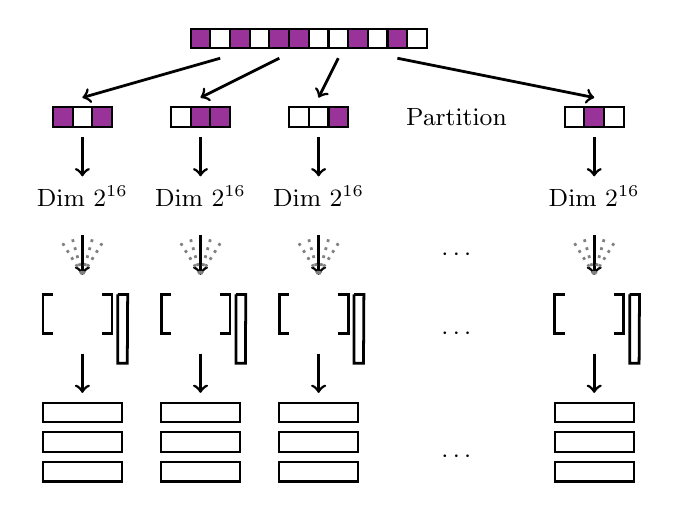
\begin{tikzpicture}
[font=\small, draw=black, line width=0.75pt,
sub0/.style={rectangle, draw, inner sep=0pt, minimum width=10mm, minimum height=2.5mm},
parity/.style={rectangle, draw, fill=cyan, inner sep=0pt, minimum size=2.5mm},
bit0/.style={rectangle, draw, inner sep=0pt, minimum size=2.5mm},
bit1/.style={rectangle, draw, fill=violet!80, inner sep=0pt, minimum size=2.5mm}]

\node[bit1] (bit0) at (0.50,8.25) {};
\node[bit0] (bit1) at (0.75,8.25) {};
\node[bit1] (bit2) at (1.00,8.25) {};
\node[bit0] (bit3) at (1.25,8.25) {};
\node[bit1] (bit4) at (1.50,8.25) {};
\node[bit1] (bit5) at (1.75,8.25) {};
\node[bit0] (bit6) at (2.00,8.25) {};
\node[bit0] (bit7) at (2.25,8.25) {};
\node[bit1] (bit8) at (2.50,8.25) {};
\node[bit0] (bit9) at (2.75,8.25) {};
\node[bit1] (bit10) at (3.00,8.25) {};
\node[bit0] (bit11) at (3.25,8.25) {};

\draw[->, line width=1pt]  (0.75,8.00) -- (-1.00,7.50);
\draw[->, line width=1pt]  (1.50,8.00) -- (0.50,7.50);
\draw[->, line width=1pt]  (2.25,8.00) -- (2.00,7.50);
\draw[->, line width=1pt]  (3.00,8.00) -- (5.50,7.50);
\node (partition) at (3.75,7.25) {Partition};

\node[bit1] (s00) at (-1.25,7.25) {};
\node[bit0] (s01) at (-1.00,7.25) {};
\node[bit1] (s02) at (-0.75,7.25) {};

\node[bit0] (s03) at (0.25,7.25) {};
\node[bit1] (s04) at (0.50,7.25) {};
\node[bit1] (s05) at (0.75,7.25) {};

\node[bit0] (s06) at (1.75,7.25) {};
\node[bit0] (s07) at (2.00,7.25) {};
\node[bit1] (s08) at (2.25,7.25) {};

\node[bit0] (s09) at (5.25,7.25) {};
\node[bit1] (s10) at (5.50,7.25) {};
\node[bit0] (s11) at (5.75,7.25) {};

\draw[->, line width=1pt]  (-1.00,7) -- (-1.00,6.5);
\draw[->, line width=1pt]  (0.50,7) -- (0.50,6.5);
\draw[->, line width=1pt]  (2.00,7) -- (2.00,6.5);
\draw[->, line width=1pt]  (5.50,7) -- (5.50,6.5);

\node (cs1) at (-1.00,6.25) {Dim~$2^{16}$};
\node (cs2) at (0.50,6.25) {Dim~$2^{16}$};
\node (cs3) at (2.00,6.25) {Dim~$2^{16}$};
\node (cs4) at (5.50,6.25) {Dim~$2^{16}$};

\foreach \v in {-1.00,0.50,2.00,5.50} {
  \draw[->, line width=1pt]  (\v,4.25) -- (\v,3.75);
  \draw[->, line width=1pt]  (\v,5.75) -- (\v,5.25);
  \draw[dotted, line width=1pt, draw=gray]  (\v-0.25,5.65) -- (\v,5.25);
  \draw[dotted, line width=1pt, draw=gray]  (\v-0.125,5.7) -- (\v,5.25);
  \draw[dotted, line width=1pt, draw=gray]  (\v+0.125,5.7) -- (\v,5.25);
  \draw[dotted, line width=1pt, draw=gray]  (\v+0.25,5.65) -- (\v,5.25);
}

\node (dots1) at (3.75,5.5) {$\cdots$};

\foreach \v in {-1.00,0.50,2.00,5.50} {
  \draw[line width=1pt] (\v-0.375,5) -- (\v-0.5,5) -- (\v-0.5,4.5) -- (\v-0.375,4.5);
  \draw[line width=1pt] (\v+0.25,5) -- (\v+0.375,5) -- (\v+0.375,4.5) -- (\v+0.25,4.5);
  \draw[line width=1pt] (\v+0.45,5) -- (\v+0.45,4.125) -- (\v+0.57,4.125) -- (\v+0.575,5) -- (\v+0.45,5);
}

\node (dots2) at (3.75,4.5) {$\cdots$};
\node (dots3) at (3.75,2.9375) {$\cdots$};

\foreach \c in {3.50, 3.125, 2.75} {
  \node[sub0] (subcs0\c) at (-1.00,\c) {};
  \node[sub0] (subcs2\c) at (0.50,\c) {};
  \node[sub0] (subcs3\c) at (2.00,\c) {};
  \node[sub0] (subcsz\c) at (5.50,\c) {};
}

\end{tikzpicture}

\end{center}
% % % % %
\begin{alertblock}{Drawbacks}
  \begin{itemize}
  \item Unordered lists of fragments
  \item Need to perform disambiguation
  \end{itemize}
\end{alertblock}
\end{frame}

% % % % % % % % % % % % % % % % % % % %

\begin{frame}
\frametitle{Fragmentation with Disambiguation}
% % % % %
\begin{center}
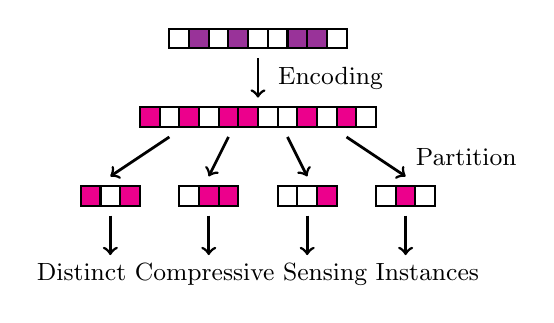
\begin{tikzpicture}
[font=\small, draw=black, line width=0.75pt,
bit0/.style={rectangle, draw, inner sep=0pt, minimum size=2.5mm},
bit1/.style={rectangle, draw, fill=violet!80, inner sep=0pt, minimum size=2.5mm},
ebit0/.style={rectangle, draw, inner sep=0pt, minimum size=2.5mm},
ebit1/.style={rectangle, draw, fill=magenta, inner sep=0pt, minimum size=2.5mm}
]

\node[bit0] (info0) at (0.875,5) {};
\node[bit1] (info1) at (1.125,5) {};
\node[bit0] (info2) at (1.375,5) {};
\node[bit1] (info3) at (1.625,5) {};
\node[bit0] (info4) at (1.875,5) {};
\node[bit0] (info5) at (2.125,5) {};
\node[bit1] (info6) at (2.375,5) {};
\node[bit1] (info7) at (2.625,5) {};
\node[bit0] (info8) at (2.875,5) {};

\draw[->, line width=1pt]  (1.875,4.75) -- (1.875,4.25);
\node[anchor=west] (coding) at (2,4.50) {Encoding};

\node[ebit1] (ebit0) at (0.50,4) {};
\node[ebit0] (ebit1) at (0.75,4) {};
\node[ebit1] (ebit2) at (1.00,4) {};
\node[ebit0] (ebit3) at (1.25,4) {};
\node[ebit1] (ebit4) at (1.50,4) {};
\node[ebit1] (ebit5) at (1.75,4) {};
\node[ebit0] (ebit6) at (2.00,4) {};
\node[ebit0] (ebit7) at (2.25,4) {};
\node[ebit1] (ebit8) at (2.50,4) {};
\node[ebit0] (ebit9) at (2.75,4) {};
\node[ebit1] (ebit10) at (3.00,4) {};
\node[ebit0] (ebit11) at (3.25,4) {};

\draw[->, line width=1pt]  (0.75,3.75) -- (0.00,3.25);
\draw[->, line width=1pt]  (1.50,3.75) -- (1.25,3.25);
\draw[->, line width=1pt]  (2.25,3.75) -- (2.50,3.25);
\draw[->, line width=1pt]  (3.00,3.75) -- (3.75,3.25);
\node[anchor=west] (coding) at (3.75,3.50) {Partition};

\node[ebit1] (s00) at (-0.25,3.00) {};
\node[ebit0] (s01) at (0.00,3.00) {};
\node[ebit1] (s02) at (0.25,3.00) {};

\node[ebit0] (s03) at (1.00,3.00) {};
\node[ebit1] (s04) at (1.25,3.00) {};
\node[ebit1] (s05) at (1.50,3.00) {};

\node[ebit0] (s06) at (2.25,3.00) {};
\node[ebit0] (s07) at (2.50,3.00) {};
\node[ebit1] (s08) at (2.75,3.00) {};

\node[ebit0] (s09) at (3.50,3.00) {};
\node[ebit1] (s10) at (3.75,3.00) {};
\node[ebit0] (s11) at (4.00,3.00) {};

\draw[->, line width=1pt]  (0.00,2.75) -- (0.00,2.25);
\draw[->, line width=1pt]  (1.25,2.75) -- (1.25,2.25);
\draw[->, line width=1pt]  (2.50,2.75) -- (2.50,2.25);
\draw[->, line width=1pt]  (3.75,2.75) -- (3.75,2.25);

\node (cs) at (1.875,2.00) {Distinct Compressive Sensing Instances};
\end{tikzpicture}

\end{center}
% % % % %
\vfill
% % % % %
\begin{block}{Stitching through outer code}
\begin{itemize}
\item Split problem into sub-components suitable for CS framework
\item Get lists of sub-packets, one list for every slot
\item Stitch pieces of one packet together using error correction
\end{itemize}
\end{block}
\end{frame}

% % % % % % % % % % % % % % % % % % % %

\begin{frame}
\frametitle{Coded Compressive Sensing -- Device Perspective}
% % % % %
\begin{center}
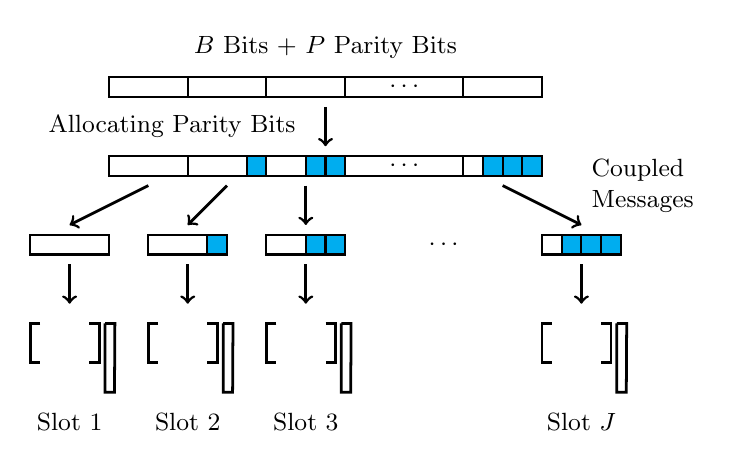
\begin{tikzpicture}
[font=\small, draw=black, line width=0.75pt,
sub0/.style={rectangle, draw, inner sep=0pt, minimum width=10mm,  minimum height=2.5mm},
sub1/.style={rectangle, draw, inner sep=0pt, minimum width=15mm, minimum height=2.5mm},
sub1s/.style={rectangle, inner sep=0pt, minimum width=15mm, minimum height=2.5mm},
parity/.style={rectangle, draw, fill=cyan, inner sep=0pt, minimum size=2.5mm}]

\node (coupledvector) at (2.25,5.50) {$B$~Bits + $P$~Parity Bits};
\node[sub0] (cs0) at (0.00,5) {};
\node[sub0] (cs2) at (1.00,5) {};
\node[sub0] (cs3) at (2.00,5) {};
\node[sub1] (csx) at (3.25,5) {$\cdots$};
\node[sub0] (csz) at (4.50,5) {};

\draw[->, line width=1pt]  (2.25,4.75) -- (2.25,4.25);
\node[anchor=east] (coding) at (2.00,4.50) {Allocating Parity Bits};

\node[sub0] (subcs0) at (0.00,4) {};
\node[sub0] (subcs2) at (1.00,4) {};
\node[parity] (parity0) at (1.375,4) {};
\node[sub0] (subcs3) at (2.00,4) {};
\node[parity] (parity1) at (2.125,4) {};
\node[parity] (parity2) at (2.375,4) {};
\node[sub1] (subcsx) at (3.25,4) {$\cdots$};
\node[sub0] (subcsz) at (4.50,4) {};
\node[parity] (parity3) at (4.375,4) {};
\node[parity] (parity4) at (4.625,4) {};
\node[parity] (parity5) at (4.875,4) {};

\node[sub0] (subcs0) at (-1.00,3) {};
\node[sub0] (subcs2) at (0.50,3) {};
\node[parity] (parity0) at (0.875,3) {};
\node[sub0] (subcs3) at (2.00,3) {};
\node[parity] (parity1) at (2.125,3) {};
\node[parity] (parity2) at (2.375,3) {};
\node[sub1s] (subcsx) at (3.75,3) {$\cdots$};
\node[sub0] (subcsz) at (5.50,3) {};
\node[parity] (parity3) at (5.375,3) {};
\node[parity] (parity4) at (5.625,3) {};
\node[parity] (parity5) at (5.875,3) {};

\draw[->, line width=1pt]  (0.00,3.75) -- (-1.00,3.25);
\draw[->, line width=1pt]  (1.00,3.75) -- (0.50,3.25);
\draw[->, line width=1pt]  (2.00,3.75) -- (2.00,3.25);
\draw[->, line width=1pt]  (4.50,3.75) -- (5.50,3.25);
\node[anchor=west,align=left] (coupledvector) at (5.50,3.75) {Coupled\\Messages};

\foreach \v in {-1.00,0.50,2.00,5.50} {
  \draw[->, line width=1pt]  (\v,2.75) -- (\v,2.25);

  \draw[line width=1pt] (\v-0.375,2) -- (\v-0.5,2) -- (\v-0.5,1.5) -- (\v-0.375,1.5);
  \draw[line width=1pt] (\v+0.25,2) -- (\v+0.375,2) -- (\v+0.375,1.5) -- (\v+0.25,1.5);
  \draw[line width=1pt] (\v+0.45,2) -- (\v+0.45,1.125) -- (\v+0.57,1.125) -- (\v+0.575,2) -- (\v+0.45,2);
}

\node (cs) at (-1.00,0.75) {Slot~1};
\node (cs) at (0.50,0.75) {Slot~2};
\node (cs) at (2.00,0.75) {Slot~3};
\node (cs) at (5.50,0.75) {Slot~$J$};
\end{tikzpicture}

\end{center}
% % % % %
\begin{itemize}
\item Collection of $L$ CS matrices and 1-sparse vectors
\item Each CS generated signal is sent in specific time slot
\end{itemize}
\myfootnote{\tiny
V. K. Amalladinne, J.-F. Chamberland, and K. R. Narayanan. \emph{A coded compressed sensing scheme for unsourced multiple access}. IEEE Transactions on Information Theory, 2020.}
\end{frame}

% % % % % % % % % % % % % % % % % % % %

\begin{frame}
\frametitle{Coded Compressive Sensing -- Multiple Access}
% % % % %
\begin{center}
\begin{tikzpicture}
[font=\small, draw=black, line width=0.75pt, >=stealth',
sub0/.style={rectangle, draw, inner sep=0pt, minimum width=10mm, minimum height=2.5mm},
parity/.style={rectangle, draw, fill=teal, inner sep=0pt, minimum size=2.5mm}]

\node (cs1) at (-1.00,6.125) {Slot~1};
\node (cs2) at (0.50,6.125) {Slot~2};
\node (cs3) at (2.00,6.125) {Slot~3};
\node (cs4) at (5.50,6.125) {Slot~$L$};

\foreach \v in {-1.00,0.50,2.00,5.50} {
  \draw[->, line width=1pt]  (\v,3.875) -- (\v,3.375);
  \draw[->, line width=1pt]  (\v,5.75) -- (\v,5.25);
  \draw[dotted, line width=1pt, draw=gray]  (\v-0.25,5.65) -- (\v,5.25);
  \draw[dotted, line width=1pt, draw=gray]  (\v-0.125,5.7) -- (\v,5.25);
  \draw[dotted, line width=1pt, draw=gray]  (\v+0.125,5.7) -- (\v,5.25);
  \draw[dotted, line width=1pt, draw=gray]  (\v+0.25,5.65) -- (\v,5.25);
}

\node (dots1) at (3.75,5.5) {$\cdots$};

\foreach \v in {-1.00,0.50,2.00,5.50} {
  \draw[line width=1pt] (\v-0.375,5) -- (\v-0.5,5) -- (\v-0.5,4.5) -- (\v-0.375,4.5);
  \draw[line width=1pt] (\v+0.25,5) -- (\v+0.375,5) -- (\v+0.375,4.5) -- (\v+0.25,4.5);
  \draw[line width=1pt] (\v+0.45,5) -- (\v+0.45,4.125) -- (\v+0.57,4.125) -- (\v+0.575,5) -- (\v+0.45,5);
}

\node (dots2) at (3.75,4.5) {$\cdots$};
\node (dots3) at (3.75,2.25) {$\cdots$};

\foreach \c in {3.00, 2.625, 2.25, 1.875, 1.5} {
  \node[sub0] (subcs0\c) at (-1.00,\c) {};
  \node[sub0] (subcs2\c) at (0.50,\c) {};
  \node[parity] (parity0\c) at (0.875,\c) {};
  \node[sub0] (subcs3\c) at (2.00,\c) {};
  \node[parity] (parity1\c) at (2.125,\c) {};
  \node[parity] (parity2\c) at (2.375,\c) {};
  \node[sub0] (subcsz\c) at (5.50,\c) {};
  \node[parity] (parity3\c) at (5.375,\c) {};
  \node[parity] (parity4\c) at (5.625,\c) {};
  \node[parity] (parity5\c) at (5.875,\c) {};
}

\node (list1) at (-1.00,1) {List~1};
\node (list2) at (0.50,1) {List~2};
\node (list3) at (2.00,1) {List~3};
\node (list4) at (5.50,1) {List~$L$};
\end{tikzpicture}

\end{center}
% % % % %
\begin{itemize}
\item $L$ instances of CS problem, each solved with non-negative LS
\item Produces $L$ lists of $K$ decoded sub-packets (with parity)
\item Must piece sub-packets together using tree decoder
\end{itemize}
\end{frame}

% % % % % % % % % % % % % % % % % % % %

\begin{frame}
\frametitle{Coded Compressive Sensing -- Stitching Process}
% % % % %
\begin{center}
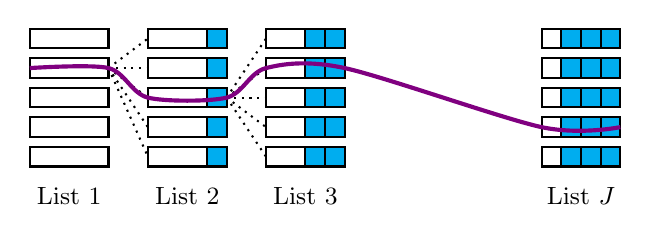
\begin{tikzpicture}
[font=\small, draw=black, line width=0.75pt,
sub0/.style={rectangle, draw, inner sep=0pt, minimum width=10mm, minimum height=2.5mm},
parity/.style={rectangle, draw, fill=cyan, inner sep=0pt, minimum size=2.5mm}]

\foreach \c in {3.00, 2.625, 2.25, 1.875, 1.5} {
  \node[sub0] (subcs1\c) at (-1.00,\c) {};
  \node[sub0] (subcs2\c) at (0.50,\c) {};
  \node[parity] (parity0\c) at (0.875,\c) {};
  \node[sub0] (subcs3\c) at (2.00,\c) {};
  \node[parity] (parity1\c) at (2.125,\c) {};
  \node[parity] (parity2\c) at (2.375,\c) {};
  \node[sub0] (subcsz\c) at (5.50,\c) {};
  \node[parity] (parity3\c) at (5.375,\c) {};
  \node[parity] (parity4\c) at (5.625,\c) {};
  \node[parity] (parity5\c) at (5.875,\c) {};
}

\draw[dotted] (-0.50,2.625) -- (0.00,3.00) {};
\draw[dotted] (-0.50,2.625) -- (0.00,2.625) {};
\draw[dotted] (-0.50,2.625) -- (0.00,2.25) {};
\draw[dotted] (-0.50,2.625) -- (0.00,1.875) {};
\draw[dotted] (-0.50,2.625) -- (0.00,1.50) {};

\draw[dotted] (1.00,2.25) -- (1.50,3.00) {};
\draw[dotted] (1.00,2.25) -- (1.50,2.625) {};
\draw[dotted] (1.00,2.25) -- (1.50,2.25) {};
\draw[dotted] (1.00,2.25) -- (1.50,1.875) {};
\draw[dotted] (1.00,2.25) -- (1.50,1.50) {};

\node (list1) at (-1.00,1) {List~1};
\node (list2) at (0.50,1) {List~2};
\node (list3) at (2.00,1) {List~3};
\node (list4) at (5.50,1) {List~$J$};

\draw [line width=1.5pt,color=violet] plot[smooth, tension=.5] coordinates {
(-1.50,2.625) (-0.50,2.625)
(0.00,2.25) (1.00,2.25)
(1.50,2.625) (2.50,2.625)
(5.00, 1.875) (6.00, 1.875)};
\end{tikzpicture}

\end{center}
% % % % %
\begin{columns}
\column{.45\textwidth}
\begin{block}{Tree decoding principles}
  \begin{itemize}
  \item Every parity is linear combination of bits in preceding blocks
  \item Late parity bits offer better performance
  \item Early parity bits decrease decoding complexity
  \item Correct fragment is on list
  \end{itemize}
\end{block}
\column{.45\textwidth}
  \centerline{\scalebox{0.5}{\begin{tikzpicture}
  [
  line width=1pt, draw=black, >=stealth',
  checknode/.style={circle, inner sep=0pt, minimum size=5mm, draw=black}
  ]

  \node[checknode, draw=darkgray] (b1) at (0,4) {};

  \foreach \x in {1,2,3} {
    \node[checknode] (c1\x) at (-6+3*\x,2) {}
      edge[<-] (b1);
  }

  \foreach \y in {1,2,3,4,5} {
    \node[checknode] (b1\y) at (-4.8+0.6*\y,0) {}
      edge[<-] (c11)
      edge[-,dotted] (-4.8+0.6*\y,-0.5);
    \node[checknode] (b2\y) at (-1.8+0.6*\y,0) {}
      edge[<-] (c12)
      edge[-,dotted] (-1.8+0.6*\y,-0.5);
    \node[checknode] (b3\y) at (1.2+0.6*\y,0) {}
      edge[<-] (c13)
      edge[-,dotted] (1.2+0.6*\y,-0.5);
  }
  
  \node[checknode] (c22) at (0,-2) {}
    edge[<-] (0,-1);

  \foreach \y in {1,2,3,4,5} {
    \node[checknode] (b4\y) at (-1.8+0.6*\y,-4) {}
      edge[<-] (c22);
  }

\draw [line width=1.5pt,color=blue!70!black] plot[smooth, tension=.5] coordinates {(b1.south) (c12) (b24) (c22) (b45)};
\draw [line width=1.5pt,dashed, color=blue] plot[smooth, tension=.5] coordinates {(b1.south) (c11) (b12) (-3,-2) (-4,-4)};
\end{tikzpicture}
}}
\end{columns}
\end{frame}

% % % % % % % % % % % % % % % % % % % %

\begin{frame}
\frametitle{Coded Compressive Sensing -- Understanding Parity Bits}
% % % % %
\begin{center}
\begin{tikzpicture}[
  font=\small, >=stealth',
  infobits/.style={rectangle, minimum height=6mm, minimum width=40mm, draw=black, fill=gray!10, rounded corners},
  paritybits/.style={rectangle, minimum height=6mm, minimum width=20mm, draw=black, fill=gray!20, rounded corners}
]

\node[infobits] (vb) at (2,0) {$\vec{w}$};
\node[paritybits] (vp) at (5,0) {$\vec{p}$};
\draw[|-|] (0,-0.5) to node[midway,below] {$k$ bits} (4,-0.5);
\draw[-|] (4,-0.5) to node[midway,below] {$l$ bits} (6,-0.5);
\end{tikzpicture}

\end{center}
% % % % %
\begin{itemize}
\item Consider binary information vector $\wv$ of length $k$
\item Systematically encoded using generator matrix $\Gm$, with
$\pv = \wv \Gm$
\item Suppose alternate vector $\wv_{\mathrm{r}}$ is selected at random from $\{ 0, 1 \}^k$
\end{itemize}
% % % % %
\vfill
% % % % %
\begin{block}{Lemma}
Probability that randomly selected information vector $\wv_{\mathrm{r}}$ produces same parity sub-component is given by
\begin{equation*}
\Pr (\pv = \pv_{\mathrm{r}}) = {2^{-\operatorname{rank}(\Gm)}}
\end{equation*}
\end{block}
\structure{Proof:}
%\begin{itemize}
%\item Suppose $\wv_{\mathrm{r}}$ is drawn at random from $\{ 0, 1 \}^k$
%\item Then event $\{ \pv = \pv_{\mathrm{r}} \}$ can equivalently be expressed as
%\begin{equation*}
%\begin{split}
$\{ \pv = \pv_{\mathrm{r}} \}
= \{ \wv \Gm = \wv_{\mathrm{r}} \Gm \}
= \{ \wv + \wv_{\mathrm{r}} \in \operatorname{nullspace}(\Gm) \}$
%\end{split}
%\end{equation*}
%\item Number of vectors in nullspace of $\Gm$ is $2^{\operatorname{nullity}(\Gm)} = 2^{k - \operatorname{rank} (\Gm)}$
%\item Then $\Pr ( \pv = \pv_{\mathrm{r}} )
%= \frac{2^{k - \operatorname{rank} (\Gm)}}{2^k}
%= 2^{- \operatorname{rank} (\Gm)}$
%\end{itemize}
\end{frame}

% % % % % % % % % % % % % % % % % % % %

\begin{frame}
\frametitle{Coded Compressive Sensing -- General Parity Bits}
% % % % %
\begin{center}
\begin{tikzpicture}[
  font=\footnotesize, >=stealth',
  infobits0/.style={rectangle, minimum height=6mm, minimum width=20mm, draw=black, fill=gray!10, rounded corners},
  infobits/.style={rectangle, minimum height=6mm, minimum width=12mm, draw=black, fill=gray!10, rounded corners},
  paritybits/.style={rectangle, minimum height=6mm, minimum width=8mm, draw=black, fill=gray!40, rounded corners}
]

\node[infobits0] (vb0) at (1,0) {$\wv(1)$};
\node[infobits] (vb1) at (2.6,0) {$\wv(2)$};
\node[paritybits] (vp1) at (3.6,0) {$\pv(2)$};
\node[infobits] (vb2) at (4.6,0) {$\wv(3)$};
\node[paritybits] (vp2) at (5.6,0) {$\pv(3)$};
\node[infobits] (vb3) at (6.6,0) {$\wv(4)$};
\node[paritybits] (vp3) at (7.6,0) {$\pv(4)$};
\draw[|-|] (0,-0.5) to node[midway,below] {$w_1$} (2,-0.5);
\draw[|-|] (2,-0.5) to node[midway,below] {$w_2$} (3.2,-0.5);
\draw[-|] (3.2,-0.5) to node[midway,below] {$p_2$} (4,-0.5);
\draw[|-|] (4,-0.5) to node[midway,below] {$w_3$} (5.2,-0.5);
\draw[-|] (5.2,-0.5) to node[midway,below] {$p_3$} (6,-0.5);
\draw[|-|] (6,-0.5) to node[midway,below] {$w_4$} (7.2,-0.5);
\draw[-|] (7.2,-0.5) to node[midway,below] {$p_4$} (8,-0.5);
\end{tikzpicture}

\end{center}
% % % % %
\begin{itemize}
\item True vector $(\wv_{i_1}(1), \wv_{i_1}(2), \wv_{i_1}(3), \wv_{i_1}(4))$
\item Consider alternate vector with information sub-block $(\wv_{i_1}(1), \wv_{i_2}(2), \wv_{i_3}(3), \wv_{i_4}(4))$ pieced from lists
\item To survive stage~4, candidate vector must fulfill parity equations
\end{itemize}
\begin{align*}
\left( \wv_{i_1}(1) - \wv_{i_2}(1) \right) \begin{bmatrix} \Gm_{1,2} \end{bmatrix} &= \zerov \\
\left( \wv_{i_1}(1) - \wv_{i_3}(1), \wv_{i_2}(2) - \wv_{i_3}(2) \right)
\begin{bmatrix} \Gm_{1,3} \\ \Gm_{2,3} \end{bmatrix}
&= \zerov \\
\left( \wv_{i_1}(1) - \wv_{i_4}(1), \wv_{i_2}(2) - \wv_{i_4}(2), \wv_{i_3}(3) - \wv_{i_4}(3) \right)
\begin{bmatrix} \Gm_{1,4} \\ \Gm_{2,4} \\ \Gm_{3,4} \end{bmatrix}
&= \zerov
\end{align*}
\end{frame}

% % % % % % % % % % % % % % % % % % % %

\begin{frame}
\frametitle{Coded Compressive Sensing -- General Parity Bits}
% % % % %
\begin{center}
\begin{tikzpicture}[
  font=\footnotesize, >=stealth',
  infobits0/.style={rectangle, minimum height=6mm, minimum width=20mm, draw=black, fill=gray!10, rounded corners},
  infobits/.style={rectangle, minimum height=6mm, minimum width=12mm, draw=black, fill=gray!10, rounded corners},
  paritybits/.style={rectangle, minimum height=6mm, minimum width=8mm, draw=black, fill=gray!40, rounded corners}
]

\node[infobits0] (vb0) at (1,0) {$\wv(1)$};
\node[infobits] (vb1) at (2.6,0) {$\wv(2)$};
\node[paritybits] (vp1) at (3.6,0) {$\pv(2)$};
\node[infobits] (vb2) at (4.6,0) {$\wv(3)$};
\node[paritybits] (vp2) at (5.6,0) {$\pv(3)$};
\node[infobits] (vb3) at (6.6,0) {$\wv(4)$};
\node[paritybits] (vp3) at (7.6,0) {$\pv(4)$};
\draw[|-|] (0,-0.5) to node[midway,below] {$w_1$} (2,-0.5);
\draw[|-|] (2,-0.5) to node[midway,below] {$w_2$} (3.2,-0.5);
\draw[-|] (3.2,-0.5) to node[midway,below] {$p_2$} (4,-0.5);
\draw[|-|] (4,-0.5) to node[midway,below] {$w_3$} (5.2,-0.5);
\draw[-|] (5.2,-0.5) to node[midway,below] {$p_3$} (6,-0.5);
\draw[|-|] (6,-0.5) to node[midway,below] {$w_4$} (7.2,-0.5);
\draw[-|] (7.2,-0.5) to node[midway,below] {$p_4$} (8,-0.5);
\end{tikzpicture}

\end{center}
% % % % %
\begin{itemize}
\item When indices are not repeated in $(\wv_{i_1}(1), \wv_{i_2}(2), \wv_{i_3}(3), \wv_{i_4}(4))$, probability is governed by
\begin{equation*}
\operatorname{rank}
\left(
\begin{bmatrix}
\Gm_{1,2} & \Gm_{1,3} & \Gm_{1,4} \\
\mathbf{0} & \Gm_{2,3} & \Gm_{2,4} \\
\mathbf{0} & \mathbf{0}& \Gm_{3,4}
\end{bmatrix}
\right)
\end{equation*}
\item But, when indices are repeated, sub-blocks may disappear
\begin{equation*}
\operatorname{rank}
\left(
\begin{bmatrix}
\Gm_{1,2} \mathbf{1}_{\{ i_2 \neq i_1 \}} & \Gm_{1,3} \mathbf{1}_{\{ i_3 \neq i_1 \}} & \Gm_{1,4} \mathbf{1}_{\{ i_4 \neq i_1 \}} \\
\mathbf{0} & \Gm_{2,3} \mathbf{1}_{\{ i_3 \neq i_2 \}} & \Gm_{2,4} \mathbf{1}_{\{ i_4 \neq i_2 \}} \\
\mathbf{0} & \mathbf{0}& \Gm_{3,4} \mathbf{1}_{\{ i_4 \neq i_3 \}}
\end{bmatrix}
\right)
\end{equation*}
\end{itemize}
\end{frame}

% % % % % % % % % % % % % % % % % % % %

\begin{frame}
\frametitle{Candidate Paths and Bell Numbers}
% % % % %
\begin{columns}
\column{0.55\textwidth}
  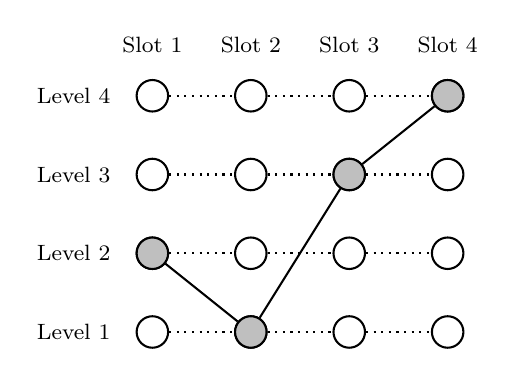
\begin{tikzpicture}
  [
  font=\footnotesize, line width=0.75pt, draw=black,
  subblock/.style={circle, inner sep = 0pt, minimum size = 4mm, draw=black}
  ]

\foreach \x in {1,2,3,4} {
  \foreach \y in {1,2,3,4} {
    \node[subblock] (x{\x}y{\y}) at (1.25*\x - 1.25,\y) {};
  }
  \node (s{\x}) at (1.25*\x - 1.25,4.65) {Slot~\x};
}
\foreach \y in {1,2,3,4} {
  \node (l{\y}) at (-1,\y) {Level~\y};
}

\foreach \y in {1,2,3,4} {
  \draw[dotted](x{1}y{\y}) -- (x{2}y{\y});
  \draw[dotted](x{2}y{\y}) -- (x{3}y{\y});
  \draw[dotted](x{3}y{\y}) -- (x{4}y{\y});
}

\node[subblock,fill=lightgray] (px1y2) at (0,2) {};
\node[subblock,fill=lightgray] (px2y1) at (1.25,1) {}
  edge (px1y2);
\node[subblock,fill=lightgray] (px3y3) at (2.5,3) {}
  edge (px2y1);
\node[subblock,fill=lightgray] (px4y4) at (3.75,4) {}
  edge (px3y3);

\end{tikzpicture}

\column{0.43\textwidth}
  Probability that wrong path is consistent with parities is
  \begin{equation*}
  \Pr (\pv = \pv_{\mathrm{r}}) = {2^{-\operatorname{rank}(\Gm)}}
  \end{equation*}
  where
  \begin{equation*}
  \Gm = \begin{bmatrix}
  \Gm_{1,2} & \Gm_{1,3} & \Gm_{1,4} \\
  \mathbf{0} & \Gm_{2,3} & \Gm_{2,4} \\
  \mathbf{0} & \mathbf{0}& \Gm_{3,4}
  \end{bmatrix}
  \end{equation*}
\end{columns}
% % % % %
\vfill
% % % % %
\begin{center}
\begin{tikzpicture}[
  font=\small, >=stealth',
  infobits0/.style={rectangle, minimum height=6mm, minimum width=20mm, draw=black, fill=gray!10, rounded corners},
  infobits/.style={rectangle, minimum height=6mm, minimum width=12mm, draw=black, fill=gray!10, rounded corners},
  paritybits/.style={rectangle, minimum height=6mm, minimum width=8mm, draw=black, fill=gray!40, rounded corners}
]

\node[infobits0] (vb0) at (1,0) {$\vec{w}(0)$};
\node[infobits] (vb1) at (2.6,0) {$\vec{w}(1)$};
\node[paritybits] (vp1) at (3.6,0) {$\vec{p}(1)$};
\node[infobits] (vb2) at (4.6,0) {$\vec{w}(2)$};
\node[paritybits] (vp2) at (5.6,0) {$\vec{p}(2)$};
\node[infobits] (vb3) at (6.6,0) {$\vec{w}(3)$};
\node[paritybits] (vp3) at (7.6,0) {$\vec{p}(3)$};
\draw[|-|] (0,-0.5) to node[midway,below] {$m_0$} (2,-0.5);
\draw[|-|] (2,-0.5) to node[midway,below] {$m_1$} (3.2,-0.5);
\draw[-|] (3.2,-0.5) to node[midway,below] {$l_1$} (4,-0.5);
\draw[|-|] (4,-0.5) to node[midway,below] {$m_2$} (5.2,-0.5);
\draw[-|] (5.2,-0.5) to node[midway,below] {$l_2$} (6,-0.5);
\draw[|-|] (6,-0.5) to node[midway,below] {$m_3$} (7.2,-0.5);
\draw[-|] (7.2,-0.5) to node[midway,below] {$l_3$} (8,-0.5);
\end{tikzpicture}
 \\[2mm]
\structure{When Levels Do NOT Repeat}
\end{center}
\end{frame}

% % % % % % % % % % % % % % % % % % % %

\begin{frame}
\frametitle{Candidate Paths and Bell Numbers}
% % % % %
\begin{columns}
\column{0.55\textwidth}
  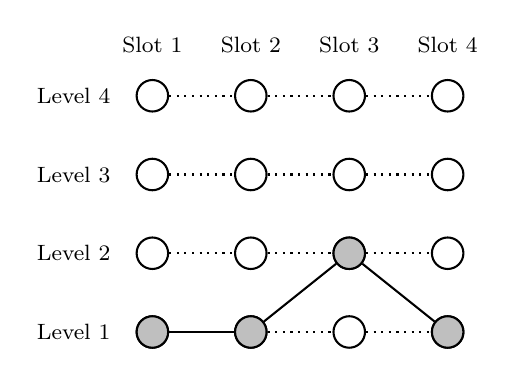
\begin{tikzpicture}
  [
  font=\footnotesize, line width=0.75pt, draw=black,
  subblock/.style={circle, inner sep = 0pt, minimum size = 4mm, draw=black}
  ]

\foreach \x in {1,2,3,4} {
  \foreach \y in {1,2,3,4} {
    \node[subblock] (x{\x}y{\y}) at (1.25*\x - 1.25,\y) {};
  }
  \node (s{\x}) at (1.25*\x - 1.25,4.65) {Slot~\x};
}
\foreach \y in {1,2,3,4} {
  \node (l{\y}) at (-1,\y) {Level~\y};
}

\foreach \y in {1,2,3,4} {
  \draw[dotted](x{1}y{\y}) -- (x{2}y{\y});
  \draw[dotted](x{2}y{\y}) -- (x{3}y{\y});
  \draw[dotted](x{3}y{\y}) -- (x{4}y{\y});
}

\node[subblock,fill=lightgray] (px1y1) at (0,1) {};
\node[subblock,fill=lightgray] (px2y1) at (1.25,1) {}
  edge (px1y1);
\node[subblock,fill=lightgray] (px3y2) at (2.5,2) {}
  edge (px2y1);
\node[subblock,fill=lightgray] (px4y1) at (3.75,1) {}
  edge (px3y2);

\end{tikzpicture}

\column{0.43\textwidth}
  Probability that wrong path is consistent with parities is
  \begin{equation*}
  \Pr (\pv = \pv_{\mathrm{r}}) = {2^{-\operatorname{rank}(\Gm)}}
  \end{equation*}
  where
  \begin{equation*}
  \Gm = \begin{bmatrix}
  \mathbf{0} & \Gm_{1,3} & \mathbf{0} \\
  \mathbf{0} & \Gm_{2,3} & \mathbf{0} \\
  \mathbf{0} & \mathbf{0}& \Gm_{3,4}
  \end{bmatrix}
  \end{equation*}
\end{columns}
% % % % %
\vfill
% % % % %
\begin{center}
\begin{tikzpicture}[
  font=\footnotesize, >=stealth',
  infobits0/.style={rectangle, minimum height=6mm, minimum width=24mm, draw=black, fill=gray!10, rounded corners},
  infobits/.style={rectangle, minimum height=6mm, minimum width=14mm, draw=black, fill=gray!10, rounded corners},
  paritybits/.style={rectangle, minimum height=6mm, minimum width=10mm, draw=black, fill=gray!40, rounded corners}
]

\node[infobits0] (vb0) at (1.2,0) {$\wv_1(1)$};
\node[infobits] (vb1) at (3.1,0) {$\wv_1(2)$};
\node[paritybits] (vp1) at (4.3,0) {$\pv_1(2)$};
\node[infobits] (vb2) at (5.5,0) {$\wv_2(3)$};
\node[paritybits] (vp2) at (6.7,0) {$\pv_2(3)$};
\node[infobits] (vb3) at (7.9,0) {$\wv_1(4)$};
\node[paritybits] (vp3) at (9.1,0) {$\pv_1(4)$};
\end{tikzpicture}
 \\[2mm]
\structure{When Levels Repeat}
\end{center}
\end{frame}

% % % % % % % % % % % % % % % % % % % %

\begin{frame}{Bell Numbers and $j$-patterns}
\begin{columns}
% % % % %
\column{0.42\textwidth}
  \begin{block}{Integer Sequences}
  \begin{itemize}
  \item $K^L$ paths
  \item Reduce complexity through equivalence
  \item Online Encyclopedia of Integer Sequences (OEIS) A000110
  \item Bell numbers grow rapidly
  \item Hard to compute expected number of surviving paths
  \end{itemize}
  \end{block}
\column{0.55\textwidth}
  \scalebox{0.75}{\begin{tikzpicture}[
  font=\scriptsize, >=stealth', line width=1.25pt, line cap=round,
  node/.style={circle, minimum size=3.25mm, inner sep=0pt, draw=black}
]

\node[node] (s1) at (0,3.1) {1};
  \node[node] (s1-1) at (1,3.1) {1};
    \node[node] (s1-1-1) at (2.5,3.1) {1};
      \node[node,label=right:{$(1,1,1,1)$}] (s1-1-1-1) at (5,3.1) {1};
      \node[node,label=right:{$(1,1,1,4)$}] (s1-1-1-4) at (5,-1.5) {3};
    \node[node] (s1-1-3) at (2.5,-0.5) {3};
      \node[node,label=right:{$(1,1,3,1)$}] (s1-1-3-1) at (5,1.9) {3};
      \node[node,label=right:{$(1,1,3,3)$}] (s1-1-3-3) at (5,-0.5) {3};
      \node[node,label=right:{$(1,1,3,4)$}] (s1-1-3-4) at (5,-2.7) {6};
  \node[node] (s1-2) at (1,0.9) {3};
    \node[node] (s1-2-1) at (2.5,2.7) {3};
      \node[node,label=right:{$(1,2,1,1)$}] (s1-2-1-1) at (5,2.7) {3};
      \node[node,label=right:{$(1,2,1,2)$}] (s1-2-1-2) at (5,0.9) {3};
      \node[node,label=right:{$(1,2,1,4)$}] (s1-2-1-4) at (5,-1.9) {6};
    \node[node] (s1-2-2) at (2.5,0.9) {3};
      \node[node,label=right:{$(1,2,2,1)$}] (s1-2-2-1) at (5,2.3) {3};
      \node[node,label=right:{$(1,2,2,2)$}] (s1-2-2-2) at (5,0.5) {3};
      \node[node,label=right:{$(1,2,2,4)$}] (s1-2-2-4) at (5,-2.3) {6};
    \node[node] (s1-2-3) at (2.5,-0.9) {6};
      \node[node,label=right:{$(1,2,3,1)$}] (s1-2-3-1) at (5,1.5) {6};
      \node[node,label=right:{$(1,2,3,2)$}] (s1-2-3-2) at (5,0.1) {6};
      \node[node,label=right:{$(1,2,3,3)$}] (s1-2-3-3) at (5,-0.9) {6};
      \node[node,label=right:{$(1,2,3,4)$}] (s1-2-3-4) at (5,-3.1) {6};

\draw[line width=0.5pt] (s1) -- (s1-1);
  \draw[line width=0.5pt] (s1-1) -- (s1-1-1);
    \draw[line width=0.5pt] (s1-1-1) -- (s1-1-1-1);
    \draw[line width=1.5pt] (s1-1-1) -- (s1-1-1-4);
  \draw[line width=1.5pt] (s1-1) -- (s1-1-3);
    \draw[line width=1.5pt] (s1-1-3) -- (s1-1-3-1);
    \draw[line width=1.5pt] (s1-1-3) -- (s1-1-3-3);
    \draw[line width=3.0pt] (s1-1-3) -- (s1-1-3-4);
\draw[line width=1.5pt] (s1) -- (s1-2);
  \draw[line width=1.5pt] (s1-2) -- (s1-2-1);
    \draw[line width=1.5pt] (s1-2-1) -- (s1-2-1-1);
    \draw[line width=1.5pt] (s1-2-1) -- (s1-2-1-2);
    \draw[line width=3.0pt] (s1-2-1) -- (s1-2-1-4);
  \draw[line width=1.5pt] (s1-2) -- (s1-2-2);
    \draw[line width=1.5pt] (s1-2-2) -- (s1-2-2-1);
    \draw[line width=1.5pt] (s1-2-2) -- (s1-2-2-2);
    \draw[line width=3.0pt] (s1-2-2) -- (s1-2-2-4);
  \draw[line width=3.0pt] (s1-2) -- (s1-2-3);
    \draw[line width=3.0pt] (s1-2-3) -- (s1-2-3-1);
    \draw[line width=3.0pt] (s1-2-3) -- (s1-2-3-2);
    \draw[line width=3.0pt] (s1-2-3) -- (s1-2-3-3);
    \draw[line width=3.0pt] (s1-2-3) -- (s1-2-3-4);

\draw[dashed] (-0.4,3.4) -- (6.8,3.4);
\draw[dashed] (-0.1,1.2) -- (6.5,1.2);
\draw[dashed] (-0.1,-0.2) -- (6.5,-0.2);
\draw[dashed] (-0.1,-1.2) -- (6.5,-1.2);
\draw[dashed] (-0.4,-3.4) -- (6.8,-3.4);

\node[rotate=90] at (-0.4,2.3) {\normalsize level~$0$};
\node[rotate=90] at (-0.4,0.5) {\normalsize level~$1$};
\node[rotate=90] at (-0.4,-0.7) {\normalsize level~$2$};
\node[rotate=90] at (-0.4,-2.3) {\normalsize level~$3$};

\node[rotate=-90] at (6.8,0) {\normalsize $j$-patterns};
\end{tikzpicture}
}
\end{columns}
% % % % %
\vfill
% % % % %
\begin{center}
\begin{tikzpicture}
\shade[draw=none,
left color={rgb:red,1;green,2;blue,3},
right color=frametitle.fg,
shading angle=60,
rounded corners,
blur shadow={shadow blur steps=5}] (-2.75,-0.625) rectangle (2.75,0.625);
\shade[fill=white, fill opacity=0.1] (-2.75,-0.625) rectangle (2.75,0.625);
\node at (0,0) {\textcolor{white}{\Large \textbf{
Need Approximation}}};
\end{tikzpicture}
\end{center}
\end{frame}

% % % % % % % % % % % % % % % % % % % %

\begin{frame}
\frametitle{Allocating Parity Bits (approximation)}
% % % % %
\begin{itemize}
\item $p_{\ell}$: \# parity bits in sub-block $\ell \in 2, \ldots, L$,
\item $P_{\ell}$: \# erroneous paths that survive stage $\ell \in 2, \ldots, L$,
\item Complexity $C_{\mathrm{tree}}$: \# nodes on which parity check constraints verified
\end{itemize}
% % % % %
\vfill
% % % % %
\begin{block}{Expressions for $\mathbb{E}[P_{\ell}]$ and $C_{\mathrm{tree}}$}
\begin{itemize}
\item $P_{\ell} \lvert P_{\ell-1} \sim B((P_{\ell-1}+1)K-1,\rho_{\ell})$, $\rho_{\ell}=2^{-p_{\ell}}$, $q_{\ell}=1-\rho_{\ell}$
\begin{align*}
\mathbb{E}[P_{\ell}] &= \mathbb{E}[ \mathbb{E}[P_{\ell} \lvert P_{\ell-1}]] \\
&= \mathbb{E}[((P_{\ell-1}+1)K-1)\rho_{\ell}] \\
&= \rho_{\ell} K\mathbb{E}[P_{\ell-1}] + \rho_{\ell}(K-1) \\
&= \sum_{r=1}^{\ell} K^{\ell-r}(K-1) \prod_{j=r}^{\ell}\rho_j
\end{align*}
\item $C_{\mathrm{tree}} = K + \sum_{\ell=2}^{L-1}\left[(P_{\ell} + 1)K\right]$
\item $\mathbb{E}[C_{\mathrm{tree}}]$ can be computed using the expression for $\mathbb{E}[P_{\ell}]$
\end{itemize}
\end{block}
\end{frame}

% % % % % % % % % % % % % % % % % % % %

\begin{frame}
\frametitle{Optimization of Parity Lengths}
% % % % %
\begin{itemize}
\item $p_{\ell}$: \# parity bits in sub-block $\ell \in 2, \ldots, L$,
\item $P_{\ell}$: \# erroneous paths that survive stage $\ell \in 2, \ldots, L$,
\end{itemize}
% % % % %
\vfill
% % % % %
\begin{block}{Relaxed geometric programming optimization}
\blockmathspace
\begin{equation*}
\begin{aligned}
& \underset{(p_2, \dots, p_{L})}{\text{minimize}}
& &\mathbb{E}[C_{\mathrm{tree}}] \\
& \text{subject to}
& & \Pr(P_{L} \ge 1) \le \varepsilon_{\mathrm{tree}}
& \text{\textcolor{frametitle.fg}{Erroneous paths}} \\
&&& \sum_{\ell=2}^{L} p_{\ell} = M-B & \text{\textcolor{frametitle.fg}{Total \# parity bits}} \\
&&& p_{\ell} \in \{ 0, \ldots, N/L \} \quad \forall~\ell \in 2, \ldots, L
& \text{\textcolor{frametitle.fg}{Integer constraints}}
\end{aligned}
\end{equation*}
\end{block}
% % % % %
\vfill
% % % % %
\begin{itemize}
\item Solved using standard convex solver, e.g., CVX
\end{itemize}
\end{frame}

% % % % % % % % % % % % % % % % % % % %

\begin{frame}
\frametitle{Choice of Parity Lengths}
% % % % %
\begin{itemize}
\item $K=200$, $L=11$, $N/L=15$
\end{itemize}
% % % % %
\vfill
% % % % %
\begin{center}
\begin{tabular}{||l|l|l||}
\hline
 $\varepsilon_{\mathrm{tree}}$ & $\mathbb{E}[C_{\mathrm{tree}}]$ & Parity Lengths $p_2, \ldots, p_L$ \\[0.5ex]
\hline \hline
$0.006$ & Infeasible & Infeasible \tabularnewline
\hline
$0.0061930$ & $3.2357\times10^{11}$ & $ 0 ,0, 0, 0, 15, 15, 15, 15, 15, 15$ \tabularnewline
\hline
$0.0061931$ & $3357300$ & $ 0, 3, 8, 8, 8, 8, 10, 15, 15, 15$ \tabularnewline
\hline
$0.0061932$ & $1737000$ & $ 0, 4, 8, 8, 8, 8, 9, 15, 15, 15$ \tabularnewline
\hline
$0.0061933$ & $926990$ & $ 0, 5, 8, 8, 8, 8, 8, 15, 15, 15$ \tabularnewline
\hline
$0.0061935$ & $467060$ & $ 1, 8, 8, 8, 8, 8, 8, 11, 15, 15$ \tabularnewline
\hline
$0.0062$ & $79634$ & $ 1, 8, 8, 8, 8, 8, 8, 11, 15, 15$ \tabularnewline
\hline
$0.007$ & $7357.8$ & $ 6, 8, 8, 8, 8, 8, 8, 8, 13, 15$ \tabularnewline
\hline
$0.008$ & $6152.7$ & $ 7, 8, 8, 8, 8, 8, 8, 8, 12, 15$ \tabularnewline
\hline
$0.02$ & $5022.9$ & $ 6, 8, 8, 9, 9, 9, 9, 9, 9, 14$ \tabularnewline
\hline
$0.04$ & $4158$ & $ 7, 8, 8, 9, 9, 9, 9, 9, 9, 13$ \tabularnewline
\hline
$0.6378$ & $3066.3$ & $ 9, 9, 9, 9, 9, 9, 9, 9, 9, 9$ \tabularnewline
\hline
\end{tabular}
\end{center}
\end{frame}

% % % % % % % % % % % % % % % % % % % %

\begin{frame}
\frametitle{Choice of Parity Lengths}
% % % % %
\begin{itemize}
\item $K=200$, $L=11$, $N/L=15$
\end{itemize}
\vfill
\begin{columns}
\column{0.45\textwidth}
\centerline{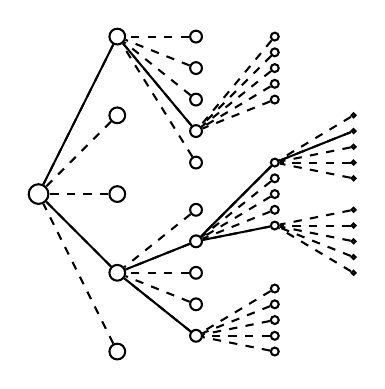
\begin{tikzpicture}
[font=\footnotesize, draw=black, line width=0.75pt,
fragment/.style={circle, draw, inner sep=0pt}]

\node[fragment,minimum size=2.5mm] (x0y0) at (0, 2) {};
\foreach \y in {0, ..., 4} {
    \node[fragment,minimum size=2mm] (x1y\y) at (1, \y) {}
        edge[dashed] (x0y0);
}
\draw (x0y0) -- (x1y4);
\draw (x0y0) -- (x1y1);

\foreach \y/\p in {51/2.4, 52/2.8, 53/3.2,  54/3.6, 55/4.0} {
    \node[fragment,minimum size=1.5mm] (x2y\y) at (2, \p) {}
        edge[dashed] (x1y4);
}
\draw (x1y4) -- (x2y52);

\foreach \y/\p in {21/0.2, 22/0.6, 23/1.0,  24/1.4, 25/1.8} {
    \node[fragment,minimum size=1.5mm] (x2y\y) at (2, \p) {}
        edge[dashed] (x1y1);
}
\draw (x1y1) -- (x2y24);
\draw (x1y1) -- (x2y21);

\foreach \y/\p in {421/3.2, 422/3.4, 423/3.6,  424/3.8, 425/4.0} {
    \node[fragment,minimum size=1mm] (x3y\y) at (3, \p) {}
        edge[dashed] (x2y52);
}

\foreach \y/\p in {241/1.6, 242/1.8, 243/2.0,  244/2.2, 245/2.4} {
    \node[fragment,minimum size=1mm] (x3y\y) at (3, \p) {}
        edge[dashed] (x2y24);
}
\draw (x2y24) -- (x3y241);
\draw (x2y24) -- (x3y245);

\foreach \y/\p in {211/0.0, 212/0.2, 213/0.4,  214/0.6, 215/0.8} {
    \node[fragment,minimum size=1mm] (x3y\y) at (3, \p) {}
        edge[dashed] (x2y21);
}

\foreach \y/\p in {2451/2.2, 2452/2.4, 2453/2.6,  2454/2.8, 2455/3.0} {
    \node[fragment,minimum size=0.5mm] (x4y\y) at (4, \p) {}
        edge[dashed] (x3y245);
}
\draw (x3y245) -- (x4y2454);

\foreach \y/\p in {2411/1.0, 2412/1.2, 2413/1.4,  2414/1.6, 2415/1.8} {
    \node[fragment,minimum size=0.5mm] (x4y\y) at (4, \p) {}
        edge[dashed] (x3y241);
}

\end{tikzpicture}}
\column{0.5\textwidth}
\begin{tabular}{|l||}
\hline
Parity Lengths $p_2, \ldots, p_L$ \\[0.5ex]
\hline \hline
$ 0 ,0, 0, 0, 15, 15, 15, 15, 15, 15$ \tabularnewline
\hline
$ 0, 3, 8, 8, 8, 8, 10, 15, 15, 15$ \tabularnewline
\hline
$ 0, 4, 8, 8, 8, 8, 9, 15, 15, 15$ \tabularnewline
\hline
$ 0, 5, 8, 8, 8, 8, 8, 15, 15, 15$ \tabularnewline
\hline
$ 1, 8, 8, 8, 8, 8, 8, 11, 15, 15$ \tabularnewline
\hline
$ 1, 8, 8, 8, 8, 8, 8, 11, 15, 15$ \tabularnewline
\hline
$ 6, 8, 8, 8, 8, 8, 8, 8, 13, 15$ \tabularnewline
\hline
$ 7, 8, 8, 8, 8, 8, 8, 8, 12, 15$ \tabularnewline
\hline
$ 6, 8, 8, 9, 9, 9, 9, 9, 9, 14$ \tabularnewline
\hline
$ 7, 8, 8, 9, 9, 9, 9, 9, 9, 13$ \tabularnewline
\hline
$ 9, 9, 9, 9, 9, 9, 9, 9, 9, 9$ \tabularnewline
\hline
\end{tabular}
\end{columns}
\end{frame}

% % % % % % % % % % % % % % % % % % % %

\begin{frame}
\frametitle{Performance of CCS and Previous Schemes}
% % % % %
\begin{center}
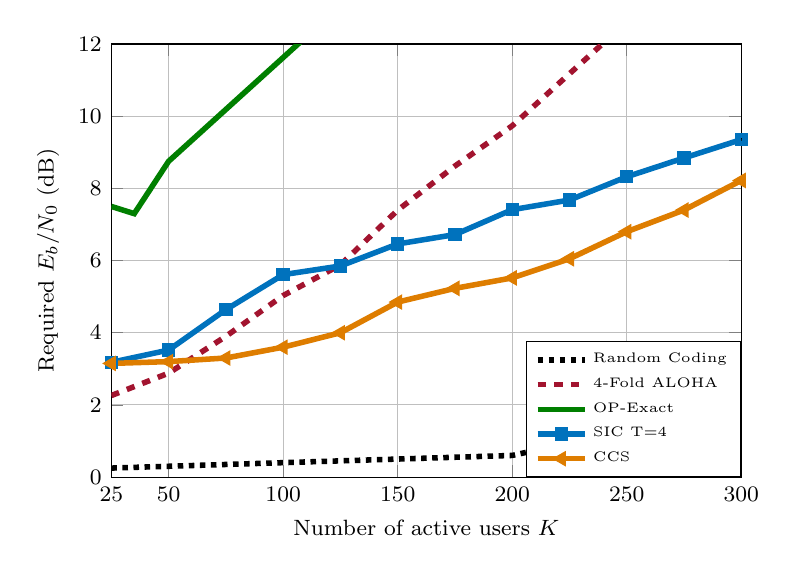
\begin{tikzpicture}
\definecolor{mycolor1}{rgb}{0.63529,0.07843,0.18431}%
\definecolor{mycolor2}{rgb}{0.00000,0.44706,0.74118}%
\definecolor{mycolor3}{rgb}{0.00000,0.49804,0.00000}%
\definecolor{mycolor4}{rgb}{0.87059,0.49020,0.00000}%
\definecolor{mycolor5}{rgb}{0.00000,0.44700,0.74100}%
\definecolor{mycolor6}{rgb}{0.74902,0.00000,0.74902}%

\begin{axis}[%
font=\footnotesize,
width=8cm,
height=5.5cm,
scale only axis,
xmin=25,
xmax=300,
xtick = {25,50,100,...,300},
xlabel={Number of active users $K$},
xmajorgrids,
ymin=0,
ymax=12,
ytick = {0,2,...,12},
ylabel={Required $E_b/N_0$ (dB)},
ylabel near ticks,
ymajorgrids,
legend style={font=\tiny, at={(1,0)},anchor=south east, draw=black,fill=white,legend cell align=left}
]

\addplot [color=black,dotted,line width=2.0pt]
  table[row sep=crcr]{
 25	0.25\\
50	0.3\\
75	0.35\\
100	0.4\\
125	0.45\\
150	0.5\\
175	0.55\\
200	0.6\\
225	0.95\\
250	1.25\\
275	1.55\\
300	1.8\\
};
\addlegendentry{Random Coding};

\addplot [color=mycolor1,dashed,line width=2.0pt]
  table[row sep=crcr]{25	2.26\\
50	2.88\\
75	3.9\\
100	5.03\\
125	5.8798\\
150	7.3954\\
175	8.6199\\
200	9.7328\\
225	11.1761\\
250	12.6127\\
275	13.3907\\
300	14.9116\\
};
\addlegendentry{4-Fold ALOHA};

\addplot [color=mycolor3,solid,line width=2.0pt]
  table[row sep=crcr]{25	7.5\\
35	7.3\\
50	8.75\\
%100	11.7\\
150	14.5\\
200	18\\
250	21\\
300	23\\
};
\addlegendentry{OP-Exact};

\addplot [color=mycolor2,solid,line width=2.0pt,mark size=1.4pt,mark=square,mark options={solid}]
  table[row sep=crcr]{25	3.18\\
50	3.52\\
75	4.64\\
100	5.61\\
125	5.85\\
150	6.46\\
175	6.72\\
200	7.41\\
225	7.6772\\
250	8.3217\\
275	8.8428\\
300	9.352\\
};
\addlegendentry{SIC T=4};

\addplot [color=mycolor4,solid,line width=2.0pt,mark size=1.3pt,mark=triangle,mark options={solid,rotate=90}]
  table[row sep=crcr]{
  25  3.15\\
50	3.2\\
75	3.3\\
100	3.6\\
125	4\\
150	4.85\\
175	5.23\\
200	5.52\\
225	6.05\\
250	6.8\\
275	7.4\\
300	8.22\\
};
\addlegendentry{CCS};

%\addplot [color=black,solid,line width=2.0pt]
%  table[row sep=crcr]{
%25	3\\
%50	3.5\\
%75  3.5\\
%100	4\\
%125	4\\
%150 4.5\\
%175 5\\
%200	5\\
%225 5.5
%250	5.8\\
%275 5.8\\
%300	6\\
%};
%\addlegendentry{AMP+Tree Code};

%\addplot [color=mycolor3,solid,line width=2.0pt,mark size=1.4pt,mark=square,mark options={solid}]
%  table[row sep=crcr]{
%  25  2\\
%50	2.1\\
%75	2.2\\
%100	2.41\\
%125	2.57\\
%150	2.81\\
%175	3\\
%200 3.4\\
%225 3.88\\
%250 4.36\\
%275 4.87\\
%300 5.35\\
%};
%\addlegendentry{Sparse IDMA};
%\node[] at (axis cs: 300,5.15) {\scriptsize \textcolor{red}{O}};
%\node[] at (axis cs: 275,4.69) {\scriptsize \textcolor{red}{O}};
%\node[] at (axis cs: 225,3.7) {\scriptsize \textcolor{red}{O}};

%\addplot [color=violet,solid,line width=2.0pt]
%  table[row sep=crcr]{
%10 0.3801\\
%20 0.5939\\
%30 0.8524\\
%40 0.9949\\
%50 1.1553\\
%60 1.3246\\
%70 1.5474\\
%80 1.7167\\
%90 1.8682\\
%100 2.0554\\
%110 2.2247\\
%120 2.3762\\
%130 2.5811\\
%140 2.7950\\
%150 2.9999\\
%160 3.1425\\
%170 3.3475\\
%180 3.5168\\
%190 3.7128\\
%200 3.8911\\
%210 4.0425\\
%220 4.2742\\
%230 4.5505\\
%240 4.7554\\
%250 4.9158\\
%260 5.0762\\
%270 5.2010\\
%280 5.3168\\
%290 5.4059\\
%300 5.4951\\
%310 5.5663\\
%320 5.6376\\
%330 5.6911\\
%340 5.7357\\
%350 5.7624\\
%360 5.7802\\
%370 5.8069\\
%380 5.8248\\
%390 5.8515\\
%400 5.9050\\
%410 6.0119\\
%420 6.1634\\
%430 6.6000\\
%};
%\addlegendentry{Polar Codes};

\end{axis}


\end{tikzpicture}%


\end{center}
\end{frame}

% % % % % % % % % % % % % % % % % % % %

\begin{frame}
\frametitle{Leveraging CCS Framework}
% % % % %
\begin{center}
\begin{tikzpicture}
  \node[scope fading=south] (image) at (0,0) {\includegraphics[width=4in]{Figures-CCS/CHIRRUP.png}};
\end{tikzpicture}
\end{center}
  \begin{itemize}
  \item Hadamard matrix based compressing scheme $+$  CSS
  \item Ultra-low complexity decoding algorithm
  \end{itemize}
\myfootnote{\tiny
S. D. Howard, A. R. Calderbank, S. J. Searle.
\emph{A Fast Reconstruction Algorithm for Deterministic Compressive Sensing using Second Order Reed-Muller Codes}. CISS 2008}
\end{frame}

% % % % % % % % % % % % % % % % % % % %

\begin{frame}
\frametitle{Example: CHIRRUP}
% % % % %
\begin{itemize}
\item Sensing matrix based on 2nd-order Reed-Muller functions,
\begin{equation*}
\phi_{R,b} (a) = \frac{(-1)^{\operatorname{wt}(b)}}{\sqrt{2^m}}
i^{(2b + Ra)^T a}
\end{equation*}
$R$ is binary symmetric matrix with zeros on diagonal, $\operatorname{wt}$ represent weight, and $i = \sqrt{-1}$
\item Every column of form
\begin{equation*}
\begin{matrix} | \\ \xv_{R,b} \\ | \end{matrix}
  = \begin{bmatrix}
  \phi_{R,b} ([0]_2) \\
  \phi_{R,b} ([1]_2) \\ \vdots \\
  \phi_{R,b} ([2^m-1]_2)
  \end{bmatrix}
\end{equation*}
$[ \cdot ]_2$ is integer expressed in radix of 2
\item Information encoded into $R$ and $b$
\item \textbf{Fast recovery:} Inner-products, Hardmard project onto Walsh basis, get $R$ row column at a time, dechirp, Hadamard project to $b$
\end{itemize}
\end{frame}
 
% % % % % % % % % % % % % % % % % % % %

\begin{frame}
\frametitle{Enhanced Coded Compressed Sensing}
\begin{center}
\begin{tikzpicture}
  \node[scope fading=south] (image) at (0,0) {\includegraphics[width=4in]{Figures-CCS/ICASSP2020.png}};
\end{tikzpicture}
\end{center}
\vfill
\begin{block}{Leverage algorithmic opportunity}
  \begin{itemize}
  \item Extending CCS framework by integrating tree code
  \item Decisions at early stages inform later parts 
  \item Algorithmic performance improvements
  \end{itemize}
\end{block}
\end{frame}

% % % % % % % % % % % % % % % % % % % %

\begin{frame}
\frametitle{Coded Compressive Sensing with Column Pruning}
\begin{center}
\begin{tikzpicture}
[font=\footnotesize, draw=black, line width=0.75pt,>=stealth',
sub0/.style={rectangle, draw, inner sep=0pt, minimum width=10mm, minimum height=2.5mm},
parity/.style={rectangle, draw, fill=teal, inner sep=0pt, minimum size=2.5mm}]

\node (cs1) at (0.00,6.125) {Slot~1};
\node (cs2) at (2.50,6.125) {Slot~2};
\node (cs3) at (5.00,6.125) {Slot~3};

\foreach \v in {0.00,2.50,5.00} {
  \draw[->, line width=1pt]  (\v,3.875) -- (\v,3.375);
  \draw[->, line width=1pt]  (\v,5.75) -- (\v,5.25);
  \draw[dotted, line width=1pt, draw=gray]  (\v-0.25,5.65) -- (\v,5.25);
  \draw[dotted, line width=1pt, draw=gray]  (\v-0.125,5.7) -- (\v,5.25);
  \draw[dotted, line width=1pt, draw=gray]  (\v+0.125,5.7) -- (\v,5.25);
  \draw[dotted, line width=1pt, draw=gray]  (\v+0.25,5.65) -- (\v,5.25);
}

\foreach \v in {0.00} {
  \draw[line width=1pt] (\v-0.5,5) -- (\v-0.625,5) -- (\v-0.625,4.5) -- (\v-0.5,4.5);
  \draw[line width=1pt] (\v+0.375,5) -- (\v+0.5,5) -- (\v+0.5,4.5) -- (\v+0.375,4.5);
  \draw[line width=1pt] (\v+0.575,5) -- (\v+0.575,3.875) -- (\v+0.695,3.875) -- (\v+0.695,5) -- (\v+0.575,5);
}

\foreach \v in {2.50,5.00} {
  \draw[line width=1pt] (\v-0.275,5) -- (\v-0.4,5) -- (\v-0.4,4.5) -- (\v-0.275,4.5);
  \draw[line width=1pt] (\v+0.15,5) -- (\v+0.275,5) -- (\v+0.275,4.5) -- (\v+0.15,4.5);
  \draw[line width=1pt] (\v+0.35,5) -- (\v+0.35,4.325) -- (\v+0.47,4.325) -- (\v+0.47,5) -- (\v+0.35,5);
}

\foreach \p/\c in {3.00/1, 2.625/2, 2.25/3, 1.875/4, 1.5/5} {
  \node[sub0] (subcs1\c) at (0.0,\p) {};
  \node[sub0] (subcs2\c) at (2.50,\p) {};
  \node[parity] (parity0\c) at (2.875,\p) {};
  \node[sub0] (subcs3\c) at (5.00,\p) {};
  \node[parity] (parity1\c) at (5.125,\p) {};
  \node[parity] (parity2\c) at (5.375,\p) {};
}

\node (list1) at (0.00,1) {List~1};
\node (list2) at (2.50,1) {List~2};
\node (list3) at (5.00,1) {List~3};

\draw [line width=1.5pt,color=purple,->] plot[smooth, tension=.5] coordinates {(0.5,1) (1.25,1.5) (1.375,4) (1.875,4.75)};
\draw [line width=1.5pt,color=purple,->] plot[smooth, tension=.5] coordinates {(3.0,1) (3.75,1.5) (3.875,4) (4.375,4.75)};
\draw [line width=1.5pt,color=purple,dashed] plot[smooth, tension=.5] coordinates {(5.5,1) (6.25,1.5) (6.375,4.25)};

\node[rotate=90] (prune1) at (1.0625,3) {column pruning};
\node[rotate=90] (prune2) at (3.5625,3) {column pruning};
\node[rotate=90] (prune3) at (6.0625,3) {column pruning};
\end{tikzpicture}

\end{center}
\vfill
\begin{itemize}
\item Active partial paths determine possible parity patterns
\item Admissible indices for next slot determined by possible parities
\item Inadmissible columns can be pruned before CS algorithm
\end{itemize}
\end{frame}

% % % % % % % % % % % % % % % % % % % %

%\begin{frame}
%\frametitle{Coded Compressive Sensing -- Dimensionality Reduction}
%\centerline{\begin{tikzpicture}
[font=\footnotesize, draw=black, line width=0.75pt,>=stealth',
sub0/.style={rectangle, draw, inner sep=0pt, minimum width=10mm, minimum height=2.5mm},
parity/.style={rectangle, draw, fill=teal, inner sep=0pt, minimum size=2.5mm},
star/.style={rectangle, draw, inner sep=0pt, minimum size=2.5mm},
symbol0/.style={rectangle, draw, fill=white, inner sep=0pt, minimum size=2.5mm},
symbol1/.style={rectangle, draw, fill=green!50!black, inner sep=0pt, minimum size=2.5mm}]

\foreach \v in {1.00} {
  \draw[line width=1pt] (\v-0.5,5) -- (\v-0.625,5) -- (\v-0.625,4.5) -- (\v-0.5,4.5);
  \draw[line width=1pt] (\v+0.375,5) -- (\v+0.5,5) -- (\v+0.5,4.5) -- (\v+0.375,4.5);
  \draw[line width=1pt] (\v+0.575,5) -- (\v+0.575,3.875) -- (\v+0.695,3.875) -- (\v+0.695,5) -- (\v+0.575,5);
}
\draw [line width=1.5pt,color=purple,->] (2.46,4.75) -- (3.46,4.75);

\foreach \v in {4.50} {
  \draw[line width=1pt] (\v-0.275,5) -- (\v-0.4,5) -- (\v-0.4,4.5) -- (\v-0.275,4.5);
  \draw[line width=1pt] (\v+0.15,5) -- (\v+0.275,5) -- (\v+0.275,4.5) -- (\v+0.15,4.5);
  \draw[line width=1pt] (\v+0.35,5) -- (\v+0.35,4.325) -- (\v+0.47,4.325) -- (\v+0.47,5) -- (\v+0.35,5);
}


\foreach \p/\c in {3.00/1, 2.625/2, 2.25/3, 1.875/4, 1.5/5, 1.125/6, 0.75/7} {
  \node[sub0] (subcs1\c) at (0.0,\p) {};
  \node[sub0] (subcs2\c) at (1.0,\p) {};
  \node[parity] (parity0\c) at (1.375,\p) {};
  \node[sub0] (subcs3\c) at (2.00,\p) {};
  \node[parity] (parity1\c) at (2.125,\p) {};
  \node[parity] (parity2\c) at (2.375,\p) {};
}
\node (list) at (1.00,0.25) {List of active paths};
\draw [line width=1.5pt,->] (2.75,1.875) -- (3.75,1.875);

\foreach \p/\c in {3.00/1, 2.625/2, 2.25/3, 1.875/4, 1.5/5, 1.125/6, 0.75/7} {
  \node[sub0] (subcs4\c) at (4.50,\p) {};
  \node[star] (star0\c) at (4.125,\p) {$\ast$};
  \node[star] (star1\c) at (4.375,\p) {$\ast$};
  \node[parity] (parity3\c) at (4.625,\p) {};
  \node[parity] (parity4\c) at (4.875,\p) {};
}
\node (patterns) at (4.50,0.25) {Admissible patterns};

\node[symbol0] (s01) at (7,-0.75) {};
\node[symbol1] (s02) at (7,-0.50) {};
\node[symbol0] (s03) at (7,-0.25) {};
\node[symbol1] (s04) at (7,0.00) {};
\node[symbol0] (s05) at (7,0.25) {};
\node[symbol0] (s06) at (7,0.50) {};
\node[symbol0] (s07) at (7,0.75) {};
\node[symbol1] (s08) at (7,1.00) {};
\node[symbol1] (s09) at (7,1.25) {};
\node[symbol1] (s10) at (7,1.50) {};
\node[symbol0] (s11) at (7,1.75) {};
\node[symbol1] (s12) at (7,2.00) {};
\node[symbol0] (s13) at (7,2.25) {};
\node[symbol1] (s14) at (7,2.50) {};
\node[symbol0] (s15) at (7,2.75) {};
\node[symbol1] (s16) at (7,3.00) {};
\node[symbol1] (s17) at (7,3.25) {};
\node[symbol0] (s18) at (7,3.50) {};
\node[symbol0] (s19) at (7,3.75) {};
\node[symbol1] (s20) at (7,4.00) {};
\node[symbol0] (s21) at (7,4.25) {};
\node[symbol1] (s22) at (7,4.50) {};
\node[symbol0] (s23) at (7,4.75) {};
\node[symbol1] (s24) at (7,5.00) {};
\node[rotate=-90] (indices) at (7.5,2.125) {Possible indices};

\draw[->,shorten <=1mm,shorten >=1mm]  (parity42.east) -- (s02.west);
\draw[->,shorten <=1mm,shorten >=1mm]  (parity45.east) -- (s04.west);
\draw[->,shorten <=1mm,shorten >=1mm]  (parity44.east) -- (s08.west);
\draw[->,shorten <=1mm,shorten >=1mm]  (parity41.east) -- (s09.west);
\draw[->,shorten <=1mm,shorten >=1mm]  (parity41.east) -- (s10.west);
\draw[->,shorten <=1mm,shorten >=1mm]  (parity46.east) -- (s12.west);
\draw[->,shorten <=1mm,shorten >=1mm]  (parity45.east) -- (s14.west);
\draw[->,shorten <=1mm,shorten >=1mm]  (parity42.east) -- (s16.west);
\draw[->,shorten <=1mm,shorten >=1mm]  (parity43.east) -- (s17.west);
\draw[->,shorten <=1mm,shorten >=1mm]  (parity43.east) -- (s20.west);
\draw[->,shorten <=1mm,shorten >=1mm]  (parity46.east) -- (s22.west);
\draw[->,shorten <=1mm,shorten >=1mm]  (parity44.east) -- (s24.west);
\draw[->,shorten <=1mm,shorten >=1mm]  (parity47.east) -- (s17.west);
\draw[->,shorten <=1mm,shorten >=1mm]  (parity47.east) -- (s20.west);

\end{tikzpicture}
}
%\begin{itemize}
%\item Every surviving path produces parity pattern
%\item Only fragments with these pattern can appear in subsequent slot
%\item On average, there are $K (1 + \mathrm{E}[P_{\ell}])$ possibilities parity patterns
%\end{itemize}
%\end{frame}

% % % % % % % % % % % % % % % % % % % %

\begin{frame}
\frametitle{Coded Compressive Sensing with Column Pruning}
\begin{center}
\input{Figures-CCS/eCCS3}
\end{center}
\vfill
\begin{itemize}
\item For $K$ small, width of sensing matrix is greatly reduced
\item Actual sensing matrix is determined dynamically at run time
\item Complexity of CS algorithm becomes much smaller
\end{itemize}
\end{frame}

% % % % % % % % % % % % % % % % % % % %

\begin{frame}
\frametitle{Expected Column Reduction Ratio}
\begin{columns}
\column{0.6\textwidth}
  \centerline{\scalebox{0.9}{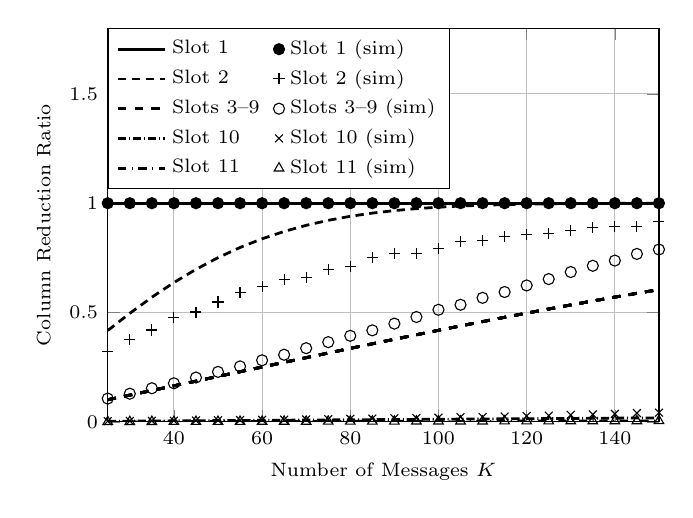
\begin{tikzpicture}

\begin{axis}[%
font=\scriptsize,
width=7cm,
height=5cm,
scale only axis,
xmin=25,
xmax=150,
xlabel={Number of Messages $K$},
xmajorgrids,
ymin=0,
ymax=1.8,
ylabel={Column Reduction Ratio},
ylabel near ticks,
ymajorgrids,
legend columns=2, 
legend style={at={(0,1)},anchor=north west,legend cell align=left,
/tikz/column 2/.style={column sep=3pt}}
]

\addplot [color=black,solid,line width=1.0pt]
  coordinates {
(25, 1.00000) (30, 1.00000) (35, 1.00000) (40, 1.00000) (45, 1.00000) (50, 1.00000) (55, 1.00000) (60, 1.00000) (65, 1.00000) (70, 1.00000) (75, 1.00000) (80, 1.00000) (85, 1.00000) (90, 1.00000) (95, 1.00000) (100, 1.00000) (105, 1.00000) (110, 1.00000) (115, 1.00000) (120, 1.00000) (125, 1.00000) (130, 1.00000) (135, 1.00000) (140, 1.00000) (145, 1.00000) (150, 1.00000)
};
\addlegendentry{Slot 1};

\addplot [only marks,mark=*]
  coordinates {
(25, 1.00000) (30, 1.00000) (35, 1.00000) (40, 1.00000) (45, 1.00000) (50, 1.00000) (55, 1.00000) (60, 1.00000) (65, 1.00000) (70, 1.00000) (75, 1.00000) (80, 1.00000) (85, 1.00000) (90, 1.00000) (95, 1.00000) (100, 1.00000) (105, 1.00000) (110, 1.00000) (115, 1.00000) (120, 1.00000) (125, 1.00000) (130, 1.00000) (135, 1.00000) (140, 1.00000) (145, 1.00000) (150, 1.00000)
};
\addlegendentry{Slot 1 (sim)};

\addplot [color=black,densely dashed,line width=1.0pt]
  coordinates {
(25, 0.41804) (30, 0.49668) (35, 0.57002) (40, 0.63716) (45, 0.69757) (50, 0.75100) (55, 0.79749) (60, 0.83732) (65, 0.87092) (70, 0.89882) (75, 0.92167) (80, 0.94010) (85, 0.95475) (90, 0.96624) (95, 0.97511) (100, 0.98188) (105, 0.98697) (110, 0.99075) (115, 0.99351) (120, 0.99550) (125, 0.99692) (130, 0.99792) (135, 0.99861) (140, 0.99908) (145, 0.99940) (150, 0.99961)
};
%curve below is generate using the PMF of #erroneous paths
%coordinates {
%(25, 0.3254) (30, 0.3765) (35, 0.4237) (40, 0.4674) (45, 0.5077) (50, 0.5450) (55, 0.5794) (60, 0.6113) (65, 0.6407) (70, 0.6679) (75, 0.6931) (80, 0.7163) (85, 0.7378) (90, 0.7576) (95, 0.7760) (100, 0.7930) (105, 0.8086) (110, 0.8231) (115, 0.8365) (120, 0.8489) (125, 0.8603) (130, 0.8709) (135, 0.8807) (140, 0.8897) (145, 0.8981) (150, 0.9058)
%};
\addlegendentry{Slot 2};

\addplot [only marks,mark=+]
  coordinates {
(25,0.3218750) (30,0.3773437) (35,4.203125e-01) (40,4.765625e-01) (45,5.023437e-01) (50,5.484375e-01) (55,5.898438e-01) (60,6.171875e-01) (65,6.515625e-01)
(70,6.585937e-01) (75,6.953125e-01) (80,7.117187e-01) (85,7.523437e-01) (90,7.695313e-01) (95,7.703125e-01)
(100,7.929688e-01) (105,8.250000e-01) (110,8.296875e-01) (115,8.484375e-01) (120,8.578125e-01)(125,8.609e-01)(130,8.734e-01)(135,8.8906e-01)(140,8.9218e-01)(145,8.9375e-01)(150,9.1562e-01)

};
\addlegendentry{Slot 2 (sim)};

\addplot [color=black,dashed,line width=1.0pt]
  coordinates {
(25, 0.10149) (30, 0.12253) (35, 0.14374) (40, 0.16507) (45, 0.18649) (50, 0.20797) (55, 0.22947) (60, 0.25095) (65, 0.27240) (70, 0.29377) (75, 0.31504) (80, 0.33617) (85, 0.35715) (90, 0.37794) (95, 0.39851) (100, 0.41885) (105, 0.43893) (110, 0.45873) (115, 0.47823) (120, 0.49741) (125, 0.51626) (130, 0.53476) (135, 0.55289) (140, 0.57064) (145, 0.58800) (150, 0.60497)
};
%coordinates {
%(25,0.0932) (30,0.1108)    (35,0.1280)    (40,0.1449)    (45,0.1615)    (50,0.1777)    (55,0.1937)    (60,0.2093)    (65,0.2246)    (70,0.2396)    (75,0.2544)  (80,0.2688)    (85,0.2830)    (90,0.2969)    (95,0.3105)    (100,0.3239)    (105,0.3370)    (110,0.3498)    (115,0.3624)    (120,0.3748)    (125,0.3869)    (130,0.3988) (135,0.4104)    (140,0.4219)    (145,0.4331)    (150,0.4441) 
%};
\addlegendentry{Slots 3--9};

\addplot [only marks,mark=o]
  coordinates {(25,1.067801e-01) (30,1.290179e-01) (35,1.539342e-01) (40,1.766462e-01) (45,2.029297e-01) (50,2.287109e-01) (55,2.539342e-01) (60,2.817243e-01) (65,3.071429e-01)
(70,3.371094e-01) (75,3.647879e-01) (80,3.937221e-01) (85,4.186663e-01) (90,4.494420e-01) (95,4.797433e-01)
(100,5.127511e-01) (105,5.356027e-01) (110,5.672991e-01) (115,5.939732e-01) (120,6.239955e-01)(125,6.5306e-01)(130,6.8526e-01)(135,7.1395e-01)(140,7.3766e-01)(145,7.6813e-01)(150,7.8825e-01)
};
\addlegendentry{Slots 3--9 (sim)};

\addplot [color=black,densely dashdotted,line width=1.0pt]
  coordinates {
(25, 0.00306) (30, 0.00367) (35, 0.00428) (40, 0.00489) (45, 0.00551) (50, 0.00612) (55, 0.00674) (60, 0.00735) (65, 0.00797) (70, 0.00858) (75, 0.00920) (80, 0.00981) (85, 0.01043) (90, 0.01104) (95, 0.01166) (100, 0.01228) (105, 0.01290) (110, 0.01352) (115, 0.01413) (120, 0.01475) (125, 0.01537) (130, 0.01599) (135, 0.01661) (140, 0.01723) (145, 0.01785) (150, 0.01847)
};
%coordinates {
% (25,0.0030)    (30,0.0037)    (35,0.0043)    (40,0.0049)    (45,0.0055)    (50,0.0061)    (55,0.0067)    (60,0.0073)    (65,0.0079)    (70,0.0085)    (75,0.0091)
%    (80,0.0097)    (85,0.0103)    (90,0.0109)    (95,0.0115)    (100,0.0121)    (105,0.0127)    (110,0.0133)    (115,0.0139)    (120,0.0145)    (125,0.0151)    (130,0.0157)  
%    (135,0.0163)    (140,0.0169)    (145,0.0175)    (150,0.0181)  
%};
\addlegendentry{Slot 10};

\addplot [only marks,mark=x]
  coordinates {(25,3.332520e-03) (30,4.180908e-03) (35,4.901123e-03) (40,5.511475e-03) (45,6.542969e-03) (50,7.434082e-03) (55,8.605957e-03) (60,9.436035e-03) (65,1.044312e-02)
 (70,1.149292e-02) (75,1.278687e-02) (80,1.430054e-02) (85,1.522217e-02) (90,1.674194e-02) (95,1.811523e-02)
(100,1.921997e-02) (105,2.165527e-02) (110,2.257080e-02) (115,2.467041e-02) (120,2.714844e-02)(125,2.8845e-02)(130,3.2532e-02)(135,3.4167e-02)(140,3.6804e-02)(145,4.0258e-02)(150,4.2333e-02)
};
\addlegendentry{Slot 10 (sim)};

\addplot [color=black,dashdotted,line width=1.0pt]
  coordinates {
(25, 0.00076) (30, 0.00092) (35, 0.00107) (40, 0.00122) (45, 0.00137) (50, 0.00153) (55, 0.00168) (60, 0.00183) (65, 0.00199) (70, 0.00214) (75, 0.00229) (80, 0.00244) (85, 0.00260) (90, 0.00275) (95, 0.00290) (100, 0.00306) (105, 0.00321) (110, 0.00336) (115, 0.00352) (120, 0.00367) (125, 0.00382) (130, 0.00398) (135, 0.00413) (140, 0.00428) (145, 0.00443) (150, 0.00459)
};
%coordinates{
%(25,0.0008)    (30,0.0009)    (35,0.0011)    (40,0.0014)    (45,0.0015)    (50,0.0017)    (55,0.0018)    (60,0.0020)    (65,0.0021)    (70,0.0023)    (75,0.0024)
 %   (80,0.0026)    (85,0.0028)    (90,0.0029)    (95,0.0031)    (100,0.0032)    (105,0.0034)    (110,0.0035)    (115,0.0037)    (120,0.0038)    (125,0.0040)    (130,0.0041)  
  %  (135,0.0043)    (140,0.0044)    (145,0.0046)    (150,0.0047)
%}
\addlegendentry{Slot 11};

\addplot [only marks,mark=triangle]
  coordinates {(25,7.644653e-04) (30,9.170532e-04) (35,1.072693e-03) (40,1.228333e-03) (45,1.380920e-03) (50,1.538086e-03) (55,1.689148e-03) (60,1.841736e-03) (65,1.997375e-03)
 (70,2.151489e-03) (75,2.307129e-03) (80,2.476501e-03) (85,2.627563e-03) (90,2.786255e-03) (95,2.940369e-03)
(100,3.100586e-03) (105,3.288269e-03) (110,3.399658e-03) (115,3.573608e-03) (120,3.771973e-03)(125,3.9337e-03)(130,4.0740e-3)(135,4.2205e-03)(140,4.3854e-03)(145,4.5380e-03)(150,4.7241e-03)
};
\addlegendentry{Slot 11 (sim)};

\addplot [color=black,dashed,line width=1.0pt]
  coordinates {
(25, 0.10149) (30, 0.12253) (35, 0.14374) (40, 0.16507) (45, 0.18649) (50, 0.20797) (55, 0.22947) (60, 0.25095) (65, 0.27240) (70, 0.29377) (75, 0.31504) (80, 0.33617) (85, 0.35715) (90, 0.37794) (95, 0.39851) (100, 0.41885) (105, 0.43893) (110, 0.45873) (115, 0.47823) (120, 0.49741) (125, 0.51626) (130, 0.53476) (135, 0.55289) (140, 0.57064) (145, 0.58800) (150, 0.60497)
};

\addplot [color=black,dashed,line width=1.0pt]
  coordinates {
(25, 0.10149) (30, 0.12253) (35, 0.14374) (40, 0.16507) (45, 0.18649) (50, 0.20797) (55, 0.22947) (60, 0.25095) (65, 0.27240) (70, 0.29377) (75, 0.31504) (80, 0.33617) (85, 0.35715) (90, 0.37794) (95, 0.39851) (100, 0.41885) (105, 0.43893) (110, 0.45873) (115, 0.47823) (120, 0.49741) (125, 0.51626) (130, 0.53476) (135, 0.55289) (140, 0.57064) (145, 0.58800) (150, 0.60497)
};

\addplot [color=black,dashed,line width=1.0pt]
  coordinates {
(25, 0.10149) (30, 0.12253) (35, 0.14374) (40, 0.16507) (45, 0.18649) (50, 0.20797) (55, 0.22947) (60, 0.25095) (65, 0.27240) (70, 0.29377) (75, 0.31504) (80, 0.33617) (85, 0.35715) (90, 0.37794) (95, 0.39851) (100, 0.41885) (105, 0.43893) (110, 0.45873) (115, 0.47823) (120, 0.49741) (125, 0.51626) (130, 0.53476) (135, 0.55289) (140, 0.57064) (145, 0.58800) (150, 0.60497)
};

\addplot [color=black,dashed,line width=1.0pt]
  coordinates {
(25, 0.10149) (30, 0.12253) (35, 0.14374) (40, 0.16507) (45, 0.18649) (50, 0.20797) (55, 0.22947) (60, 0.25095) (65, 0.27240) (70, 0.29377) (75, 0.31504) (80, 0.33617) (85, 0.35715) (90, 0.37794) (95, 0.39851) (100, 0.41885) (105, 0.43893) (110, 0.45873) (115, 0.47823) (120, 0.49741) (125, 0.51626) (130, 0.53476) (135, 0.55289) (140, 0.57064) (145, 0.58800) (150, 0.60497)
};

\addplot [color=black,dashed,line width=1.0pt]
  coordinates {
(25, 0.10149) (30, 0.12253) (35, 0.14374) (40, 0.16507) (45, 0.18649) (50, 0.20797) (55, 0.22947) (60, 0.25095) (65, 0.27240) (70, 0.29377) (75, 0.31504) (80, 0.33617) (85, 0.35715) (90, 0.37794) (95, 0.39851) (100, 0.41885) (105, 0.43893) (110, 0.45873) (115, 0.47823) (120, 0.49741) (125, 0.51626) (130, 0.53476) (135, 0.55289) (140, 0.57064) (145, 0.58800) (150, 0.60497)
};

\addplot [color=black,dashed,line width=1.0pt]
  coordinates {
(25, 0.10149) (30, 0.12253) (35, 0.14374) (40, 0.16507) (45, 0.18649) (50, 0.20797) (55, 0.22947) (60, 0.25095) (65, 0.27240) (70, 0.29377) (75, 0.31504) (80, 0.33617) (85, 0.35715) (90, 0.37794) (95, 0.39851) (100, 0.41885) (105, 0.43893) (110, 0.45873) (115, 0.47823) (120, 0.49741) (125, 0.51626) (130, 0.53476) (135, 0.55289) (140, 0.57064) (145, 0.58800) (150, 0.60497)
};
\end{axis}

\end{tikzpicture}
}}
\column{0.2\textwidth}
  \centerline{\begin{tikzpicture}
[font=\footnotesize, draw=black, line width=0.75pt,>=stealth']

\foreach \v in {1.00} {
  \draw[line width=1pt] (\v-0.5,5) -- (\v-0.625,5) -- (\v-0.625,4.5) -- (\v-0.5,4.5);
  \draw[line width=1pt] (\v+0.375,5) -- (\v+0.5,5) -- (\v+0.5,4.5) -- (\v+0.375,4.5);
  \draw[line width=1pt] (\v+0.575,5) -- (\v+0.575,3.875) -- (\v+0.695,3.875) -- (\v+0.695,5) -- (\v+0.575,5);
}

\draw [line width=1.5pt,color=purple,->] (1.035,3.75) -- (1.035,2.5);

\foreach \v in {1} {
  \draw[line width=1pt] (\v-0.275,2) -- (\v-0.4,2) -- (\v-0.4,1.5) -- (\v-0.275,1.5);
  \draw[line width=1pt] (\v+0.15,2) -- (\v+0.275,2) -- (\v+0.275,1.5) -- (\v+0.15,1.5);
  \draw[line width=1pt] (\v+0.35,2) -- (\v+0.35,1.325) -- (\v+0.47,1.325) -- (\v+0.47,2) -- (\v+0.35,2);
}

\end{tikzpicture}
}
\end{columns}
\begin{itemize}
\item Parity allocation parameters, with $w_{\ell} + p_{\ell} = 15$,
\begin{equation*}
(p_1, p_2, \ldots, p_{10}) = (6, 8, 8, 8, 8, 8, 8, 8, 13, 15)
\end{equation*}
\item Pruning is more pronounced at later stages
\item Effective width of sensing matrix is greatly reduced
\end{itemize}
\end{frame}

% % % % % % % % % % % % % % % % % % % %

\begin{frame}
\frametitle{Leveraging CCS Framework}
% % % % %
\begin{center}
\begin{tikzpicture}
  \node[scope fading=south] (image) at (0,0) {\includegraphics[width=4in]{Figures-CCS/CCS-MIMO.png}};
\end{tikzpicture}
\end{center}
  \begin{itemize}
  \item Activity detection in random access
  \item Massive MIMO Receiver
  \end{itemize}
\end{frame}

% % % % % % % % % % % % % % % % % % % %

\begin{frame}
\frametitle{Massive MIMO-URA}
\begin{center}
\scalebox{0.75}{\begin{tikzpicture}
  [
  font=\footnotesize, draw=black, >=stealth', line width=1.25pt,
  channel/.style={rectangle, minimum height=20mm, minimum width=15mm, draw=black, rounded corners},
  encoder/.style={rectangle, minimum height=6mm, minimum width=15mm, draw=black, rounded corners},
  decoder/.style={rectangle, minimum height=20mm, minimum width=15mm, draw=black, rounded corners},
  message/.style={rectangle, minimum height=6mm, minimum width=15mm, draw=black, rounded corners}
  ]

\foreach \e in {1,2,3,5} {
  \node[encoder] (e\e) at (2.25,3-\e) {Encoder};
}

\foreach \m in {1,2,3} {
  \node[message] (m\m) at (0.0,3-\m) {Message~${\m}$}
  edge[->] (e\m);
  \draw[<-] (m\m) -- (-1.25,3-\m);
}

\foreach \m in {5} {
  \node[message] (m\m) at (0.0,3-\m) {Message~$K$}
  edge[->] (e\m);
  \draw[<-] (m\m) -- (-1.25,3-\m);
}

\node at (0,-0.9) {$\vdots$};
\node at (2.25,-0.9) {$\vdots$};

\node[channel,align=center] (channel) at (5,0) {MIMO\\AP};
\node[decoder,align=center] (decoder) at (7.25,0) {Joint\\Decoder};
\draw[->] (channel) -- (decoder);


\draw[->] (decoder.east) -- (8.5,0);

\draw [line width=1pt,color=black,-triangle 90] plot[smooth, tension=0] coordinates {(4.25,0.8)(4,0.8)(4,1.1)};
\draw [line width=1pt,color=black,-triangle 90] plot[smooth, tension=0] coordinates {(4.25,0.4)(4,0.4)(4,0.7)};
\draw [line width=1pt,color=black,-triangle 90] plot[smooth, tension=0] coordinates {(4.25,0)(4,0)(4,0.3)};
\draw [line width=1pt,color=black,-triangle 90] plot[smooth, tension=0] coordinates {(4.25,-0.8)(4,-0.8)(4,-0.5)};

\draw[->,shorten >=8mm] (e1.east) -- (channel);
\draw[->,shorten >=8mm] (e2.east) -- (channel);
\draw[->,shorten >=8mm] (e3.east) -- (channel);
\draw[->,shorten >=8mm] (e5.east) -- (channel);

\end{tikzpicture}
}
%\scalebox{0.75}{\input{Figures-MAC/uncoordinated}}
\end{center}
\vfill
\begin{block}{Signal model}
\begin{itemize}
\item Signal received at time instant~$t$ with slot~$\ell$
\begin{equation*}
\yv(t,\ell) =
\textstyle \sum_{k=1}^K \xv_k(t,\ell) \mathbf{h}_k(\ell) + \zv(t,\ell)
%,~\xv_k = f(\wv_k) 
\end{equation*}
\item Number of receive antennas $M \gg 1$
\item Block fading -- channel does not change within CCS slot
\item Spatial correlation negligible -- $\mathbf{h}_k(\ell) \sim \mathcal{CN}(0,\mathbf{I}_M)$
\end{itemize}
\end{block}
\end{frame}

% % % % % % % % % % % % % % % % % % % %

\begin{frame}
\frametitle{Multiple Measurement Vector -- CS Interpretation}
% % % % %
\centerline{\definecolor{mycolor6}{rgb}{0.74902,0.00000,0.74902}%
\definecolor{mycolor7}{rgb}{0.87059,0.00000,0.49020}%
\definecolor{mycolor8}{rgb}{0.49020,0.00000,0.87059}%

\begin{tikzpicture}
[draw=black, line width=0.75pt,
entry0/.style={rectangle, draw, fill=white, inner sep=0pt, minimum size=2.5mm},
entry1/.style={rectangle, draw, fill=gray, inner sep=0pt, minimum size=2.5mm},
entry2/.style={rectangle, draw, fill=gray!50, inner sep=0pt, minimum size=2.5mm},
entry00/.style={rectangle, draw, fill=white, inner sep=0pt, minimum size=2.5mm},
entry11/.style={rectangle, draw, fill=gray!90, inner sep=0pt, minimum size=2.5mm},
symbol0/.style={rectangle, draw, fill=white, inner sep=0pt, minimum size=2.5mm},
symbol1/.style={rectangle, draw, fill=blue!50, inner sep=0pt, minimum size=2.5mm},
symbol2/.style={rectangle, draw, fill=blue, inner sep=0pt, minimum size=2.5mm},
symbol3/.style={rectangle, draw, fill=red!75, inner sep=0pt, minimum size=2.5mm},
symbol4/.style={rectangle, draw, fill=red!50, inner sep=0pt, minimum size=2.5mm},
symbol5/.style={rectangle, draw, fill=mycolor6, inner sep=0pt, minimum size=2.5mm},
symbol6/.style={rectangle, draw, fill=mycolor7, inner sep=0pt, minimum size=2.5mm},
symbol7/.style={rectangle, draw, fill=mycolor8, inner sep=0pt, minimum size=2.5mm}]

\node[entry0] (m0011) at (-0.50,1.50) {};
\node[entry1] (m0011) at (-0.25,1.50) {};
\node[entry0] (m0006) at (0.00,1.50) {};
\node[entry1] (m0106) at (0.25,1.50) {};
\node[entry00] (m0206) at (0.50,1.50) {};
\node[entry0] (m0306) at (0.75,1.50) {};
\node[entry0] (m0406) at (1.00,1.50) {};
\node[entry0] (m0506) at (1.25,1.50) {};
\node[entry00] (m0606) at (1.50,1.50) {};
\node[entry0] (m0706) at (1.75,1.50) {};
\node[entry0] (m0806) at (2.00,1.50) {};
\node[entry0] (m0906) at (2.25,1.50) {};

\node[entry0] (m0011) at (-0.50,1.75) {};
\node[entry0] (m0011) at (-0.25,1.75) {};
\node[entry0] (m0007) at (0.00,1.75) {};
\node[entry0] (m0107) at (0.25,1.75) {};
\node[entry00] (m0207) at (0.50,1.75) {};
\node[entry1] (m0307) at (0.75,1.75) {};
\node[entry0] (m0407) at (1.00,1.75) {};
\node[entry0] (m0507) at (1.25,1.75) {};
\node[entry00] (m0607) at (1.50,1.75) {};
\node[entry1] (m0707) at (1.75,1.75) {};
\node[entry1] (m0807) at (2.00,1.75) {};
\node[entry0] (m0907) at (2.25,1.75) {};

\node[entry00] (m0011) at (-0.50,2.00) {};
\node[entry1] (m0011) at (-0.25,2.00) {};
\node[entry0] (m0008) at (0.00,2.00) {};
\node[entry1] (m0108) at (0.25,2.00) {};
\node[entry00] (m0208) at (0.50,2.00) {};
\node[entry0] (m0308) at (0.75,2.00) {};
\node[entry0] (m0408) at (1.00,2.00) {};
\node[entry1] (m0508) at (1.25,2.00) {};
\node[entry00] (m0608) at (1.50,2.00) {};
\node[entry1] (m0708) at (1.75,2.00) {};
\node[entry0] (m0808) at (2.00,2.00) {};
\node[entry1] (m0908) at (2.25,2.00) {};

\node[entry0] (m0011) at (-0.5,2.25) {};
\node[entry0] (m0011) at (-0.25,2.25) {};
\node[entry0] (m0009) at (0.00,2.25) {};
\node[entry0] (m0109) at (0.25,2.25) {};
\node[entry11] (m0209) at (0.50,2.25) {};
\node[entry0] (m0309) at (0.75,2.25) {};
\node[entry1] (m0409) at (1.00,2.25) {};
\node[entry0] (m0509) at (1.25,2.25) {};
\node[entry00] (m0609) at (1.50,2.25) {};
\node[entry1] (m0709) at (1.75,2.25) {};
\node[entry0] (m0809) at (2.00,2.25) {};
\node[entry0] (m0909) at (2.25,2.25) {};


\node[entry1] (m0011) at (-0.5,2.5) {};
\node[entry0] (m0011) at (-0.25,2.5) {};
\node[entry1] (m0010) at (0.00,2.50) {};
\node[entry0] (m0110) at (0.25,2.50) {};
\node[entry00] (m0210) at (0.50,2.50) {};
\node[entry0] (m0310) at (0.75,2.50) {};
\node[entry0] (m0410) at (1.00,2.50) {};
\node[entry1] (m0510) at (1.25,2.50) {};
\node[entry11] (m0610) at (1.50,2.50) {};
\node[entry1] (m0710) at (1.75,2.50) {};
\node[entry0] (m0810) at (2.00,2.50) {};
\node[entry0] (m0910) at (2.25,2.50) {};

\node[entry11] (m0011) at (-0.5,2.75) {};
\node[entry0] (m0011) at (-0.25,2.75) {};
\node[entry0] (m0011) at (0.00,2.75) {};
\node[entry0] (m0111) at (0.25,2.75) {};
\node[entry00] (m0211) at (0.50,2.75) {};
\node[entry0] (m0311) at (0.75,2.75) {};
\node[entry0] (m0411) at (1.00,2.75) {};
\node[entry0] (m0511) at (1.25,2.75) {};
\node[entry11] (m0611) at (1.50,2.75) {};
\node[entry0] (m0711) at (1.75,2.75) {};
\node[entry0] (m0811) at (2.00,2.75) {};
\node[entry0] (m0911) at (2.25,2.75) {};

\node[symbol2] (g0000) at (2.75,2.75) {};
\node[entry0] (g0001) at (3,2.75) {};
\node[entry0] (g0002) at (3.25,2.75) {};
\node[entry0] (g0003) at (3.5,2.75) {};
\node[entry0] (g0004) at (3.75,2.75) {};
\node[entry0] (g0005) at (4.00,2.75) {};
\node[entry0] (g0006) at (4.25,2.75) {};
\node[entry0] (g0007) at (4.5,2.75) {};
\node[entry0] (g0008) at (4.75,2.75) {};
\node[entry0] (g0009) at (5,2.75) {};
\node[entry0] (g00091) at (5.25,2.75) {};
\node[entry0] (g00092) at (5.5,2.75) {};

\node[entry0] (g0010) at (2.75,2.5) {};
\node[entry2] (g0011) at (3,2.5) {};
\node[entry0] (g0012) at (3.25,2.5) {};
\node[entry0] (g0013) at (3.5,2.5) {};
\node[entry0] (g0014) at (3.75,2.5) {};
\node[entry0] (g0015) at (4.00,2.5) {};
\node[entry0] (g0016) at (4.25,2.5) {};
\node[entry0] (g0017) at (4.5,2.5) {};
\node[entry0] (g0018) at (4.75,2.5) {};
\node[entry0] (g0019) at (5,2.5) {};
\node[entry0] (g00191) at (5.25,2.5) {};
\node[entry0] (g00192) at (5.5,2.5) {};

\node[entry0] (g0020) at (2.75,2.25) {};
\node[entry0] (g0021) at (3,2.25) {};
\node[symbol2] (g0022) at (3.25,2.25) {};
\node[entry0] (g0023) at (3.5,2.25) {};
\node[entry0] (g0024) at (3.75,2.25) {};
\node[entry0] (g0025) at (4.00,2.25) {};
\node[entry0] (g0026) at (4.25,2.25) {};
\node[entry0] (g0027) at (4.5,2.25) {};
\node[entry0] (g0028) at (4.75,2.25) {};
\node[entry0] (g0029) at (5,2.25) {};
\node[entry0] (g00291) at (5.25,2.25) {};
\node[entry0] (g00292) at (5.5,2.25) {};

\node[entry0] (g0030) at (2.75,2) {};
\node[entry0] (g0031) at (3,2) {};
\node[entry0] (g0032) at (3.25,2) {};
\node[entry2] (g0033) at (3.5,2) {};
\node[entry0] (g0034) at (3.75,2) {};
\node[entry0] (g0035) at (4.00,2) {};
\node[entry0] (g0036) at (4.25,2) {};
\node[entry0] (g0037) at (4.5,2) {};
\node[entry0] (g0038) at (4.75,2) {};
\node[entry0] (g0039) at (5,2) {};
\node[entry0] (g00391) at (5.25,2) {};
\node[entry0] (g00392) at (5.5,2) {};

\node[entry0] (g0040) at (2.75,1.75) {};
\node[entry0] (g0041) at (3,1.75) {};
\node[entry0] (g0042) at (3.25,1.75) {};
\node[entry0] (g0043) at (3.5,1.75) {};
\node[entry2] (g0044) at (3.75,1.75) {};
\node[entry0] (g0045) at (4.00,1.75) {};
\node[entry0] (g0046) at (4.25,1.75) {};
\node[entry0] (g0047) at (4.5,1.75) {};
\node[entry0] (g0048) at (4.75,1.75) {};
\node[entry0] (g0049) at (5,1.75) {};
\node[entry0] (g00491) at (5.25,1.75) {};
\node[entry0] (g00492) at (5.5,1.75) {};

\node[entry0] (g0050) at (2.75,1.5) {};
\node[entry0] (g0051) at (3,1.5) {};
\node[entry0] (g0052) at (3.25,1.5) {};
\node[entry0] (g0053) at (3.5,1.5) {};
\node[entry0] (g0054) at (3.75,1.5) {};
\node[entry2] (g0055) at (4.00,1.5) {};
\node[entry0] (g0056) at (4.25,1.5) {};
\node[entry0] (g0057) at (4.5,1.5) {};
\node[entry0] (g0058) at (4.75,1.5) {};
\node[entry0] (g0059) at (5,1.5) {};
\node[entry0] (g00591) at (5.25,1.5) {};
\node[entry0] (g00592) at (5.5,1.5) {};

\node[entry0] (g0060) at (2.75,1.25) {};
\node[entry0] (g0061) at (3,1.25) {};
\node[entry0] (g0062) at (3.25,1.25) {};
\node[entry0] (g0063) at (3.5,1.25) {};
\node[entry0] (g0064) at (3.75,1.25) {};
\node[entry0] (g0065) at (4.00,1.25) {};
\node[symbol2] (g0066) at (4.25,1.25) {};
\node[entry0] (g0067) at (4.5,1.25) {};
\node[entry0] (g0068) at (4.75,1.25) {};
\node[entry0] (g0069) at (5,1.25) {};
\node[entry0] (g00691) at (5.25,1.25) {};
\node[entry0] (g00692) at (5.5,1.25) {};

\node[entry0] (g0070) at (2.75,1) {};
\node[entry0] (g0071) at (3,1) {};
\node[entry0] (g0072) at (3.25,1) {};
\node[entry0] (g0073) at (3.5,1) {};
\node[entry0] (g0074) at (3.75,1) {};
\node[entry0] (g0075) at (4.00,1) {};
\node[entry0] (g0076) at (4.25,1) {};
\node[symbol2] (g0077) at (4.5,1) {};
\node[entry0] (g0078) at (4.75,1) {};
\node[entry0] (g0079) at (5,1) {};
\node[entry0] (g00791) at (5.25,1) {};
\node[entry0] (g00792) at (5.5,1) {};

\node[entry0] (g0080) at (2.75,0.75) {};
\node[entry0] (g0081) at (3,0.75) {};
\node[entry0] (g0082) at (3.25,0.75) {};
\node[entry0] (g0083) at (3.5,0.75) {};
\node[entry0] (g0084) at (3.75,0.75) {};
\node[entry0] (g0085) at (4.00,0.75) {};
\node[entry0] (g0086) at (4.25,0.75) {};
\node[entry0] (g0087) at (4.5,0.75) {};
\node[entry2] (g0088) at (4.75,0.75) {};
\node[entry0] (g0089) at (5,0.75) {};
\node[entry0] (g00891) at (5.25,0.75) {};
\node[entry0] (g00892) at (5.5,0.75) {};

\node[entry0] (g0090) at (2.75,0.5) {};
\node[entry0] (g0091) at (3,0.5) {};
\node[entry0] (g0092) at (3.25,0.5) {};
\node[entry0] (g0093) at (3.5,0.5) {};
\node[entry0] (g0094) at (3.75,0.5) {};
\node[entry0] (g0095) at (4.00,0.5) {};
\node[entry0] (g0096) at (4.25,0.5) {};
\node[entry0] (g0097) at (4.5,0.5) {};
\node[entry0] (g0098) at (4.75,0.5) {};
\node[entry2] (g0099) at (5,0.5) {};
\node[entry0] (g00991) at (5.25,0.5) {};
\node[entry0] (g00992) at (5.5,0.5) {};

\node[entry0] (g0090) at (2.75,0.25) {};
\node[entry0] (g0091) at (3,0.25) {};
\node[entry0] (g0092) at (3.25,0.25) {};
\node[entry0] (g0093) at (3.5,0.25) {};
\node[entry0] (g0094) at (3.75,0.25) {};
\node[entry0] (g0095) at (4.00,0.25) {};
\node[entry0] (g0096) at (4.25,0.25) {};
\node[entry0] (g0097) at (4.5,0.25) {};
\node[entry0] (g0098) at (4.75,0.25) {};
\node[entry0] (g0099) at (5,0.25) {};
\node[symbol2] (g00991) at (5.25,0.25) {};
\node[entry0] (g00992) at (5.5,0.25) {};

\node[entry0] (g0090) at (2.75,0) {};
\node[entry0] (g0091) at (3,0) {};
\node[entry0] (g0092) at (3.25,0) {};
\node[entry0] (g0093) at (3.5,0) {};
\node[entry0] (g0094) at (3.75,0) {};
\node[entry0] (g0095) at (4.00,0) {};
\node[entry0] (g0096) at (4.25,0) {};
\node[entry0] (g0097) at (4.5,0) {};
\node[entry0] (g0098) at (4.75,0) {};
\node[entry0] (g0099) at (5,0) {};
\node[entry0] (g00991) at (5.25,0) {};
\node[entry2] (g00992) at (5.5,0) {};

\node[symbol4] (h0000) at (6,2.75) {};
\node[symbol3] (h0001) at (6.25,2.75) {};
\node[symbol4] (h0002) at (6.5,2.75) {};
\node[symbol4] (h0003) at (6.75,2.75) {};
\node[symbol3] (h0004) at (7,2.75) {};
\node[symbol4] (h0094) at (7.25,2.75) {};
\node[symbol3] (h0094) at (7.5,2.75) {};

\node[entry0] (h0010) at (6,2.5) {};
\node[entry1] (h0011) at (6.25,2.5) {};
\node[entry0] (h0012) at (6.5,2.5) {};
\node[entry11] (h0013) at (6.75,2.5) {};
\node[entry0] (h0014) at (7,2.5) {};
\node[entry0] (h0094) at (7.25,2.5) {};
\node[entry11] (h0094) at (7.5,2.5) {};

\node[symbol4] (h0020) at (6,2.25) {};
\node[symbol3] (h0021) at (6.25,2.25) {};
\node[symbol4] (h0022) at (6.5,2.25) {};
\node[symbol3] (h0023) at (6.75,2.25) {};
\node[symbol4] (h0024) at (7,2.25) {};
\node[symbol3] (h0094) at (7.25,2.25) {};
\node[symbol3] (h0094) at (7.5,2.25) {};

\node[entry11] (h0030) at (6,2) {};
\node[entry1] (h0031) at (6.25,2) {};
\node[entry00] (h0032) at (6.5,2) {};
\node[entry1] (h0033) at (6.75,2) {};
\node[entry0] (h0034) at (7,2) {};
\node[entry1] (h0094) at (7.25,2) {};
\node[entry0] (h0094) at (7.5,2) {};

\node[entry0] (h0040) at (6,1.75) {};
\node[entry1] (h0041) at (6.25,1.75) {};
\node[entry0] (h0042) at (6.5,1.75) {};
\node[entry11] (h0043) at (6.75,1.75) {};
\node[entry00] (h0044) at (7,1.75) {};
\node[entry0] (h0094) at (7.25,1.75) {};
\node[entry11] (h0094) at (7.5,1.75) {};

\node[entry0] (h0050) at (6,1.5) {};
\node[entry00] (h0051) at (6.25,1.5) {};
\node[entry11] (h0052) at (6.5,1.5) {};
\node[entry0] (h0053) at (6.75,1.5) {};
\node[entry1] (h0054) at (7,1.5) {};
\node[entry0] (h0094) at (7.25,1.5) {};
\node[entry0] (h0094) at (7.5,1.5) {};

\node[symbol4] (h0060) at (6,1.25) {};
\node[symbol3] (h0061) at (6.25,1.25) {};
\node[symbol3] (h0062) at (6.5,1.25) {};
\node[symbol4] (h0063) at (6.75,1.25) {};
\node[symbol3] (h0064) at (7,1.25) {};
\node[symbol4] (h0094) at (7.25,1.25) {};
\node[symbol4] (h0094) at (7.5,1.25) {};

\node[symbol3] (h0070) at (6,1) {};
\node[symbol4] (h0071) at (6.25,1) {};
\node[symbol4] (h0072) at (6.5,1) {};
\node[symbol3] (h0073) at (6.75,1) {};
\node[symbol4] (h0074) at (7,1) {};
\node[symbol4] (h0094) at (7.25,1) {};
\node[symbol3] (h0094) at (7.5,1) {};

\node[entry00] (h0080) at (6,0.75) {};
\node[entry1] (h0081) at (6.25,0.75) {};
\node[entry11] (h0082) at (6.5,0.75) {};
\node[entry11] (h0083) at (6.75,0.75) {};
\node[entry00] (h0084) at (7,0.75) {};
\node[entry11] (h0094) at (7.25,0.75) {};
\node[entry0] (h0094) at (7.5,0.75) {};

\node[entry11] (h0090) at (6,0.5) {};
\node[entry0] (h0091) at (6.25,0.5) {};
\node[entry1] (h0092) at (6.5,0.5) {};
\node[entry0] (h0093) at (6.75,0.5) {};
\node[entry0] (h0094) at (7,0.5) {};
\node[entry0] (h0094) at (7.25,0.5) {};
\node[entry11] (h0094) at (7.5,0.5) {};

\node[symbol4] (h0090) at (6,0.25) {};
\node[symbol4] (h0091) at (6.25,0.25) {};
\node[symbol3] (h0092) at (6.5,0.25) {};
\node[symbol4] (h0093) at (6.75,0.25) {};
\node[symbol3] (h0094) at (7,0.25) {};
\node[symbol3] (h0094) at (7.25,0.25) {};
\node[symbol3] (h0094) at (7.5,0.25) {};

\node[entry11] (h0090) at (6,0) {};
\node[entry0] (h0091) at (6.25,0) {};
\node[entry1] (h0092) at (6.5,0) {};
\node[entry0] (h0093) at (6.75,0) {};
\node[entry0] (h0094) at (7,0) {};
\node[entry1] (h0094) at (7.25,0) {};
\node[entry0] (h0094) at (7.5,0) {};

\node (equal) at (8,2) {\Large =};

\node[symbol5] (y0000) at (8.5,2.75) {};
\node[entry0] (y0001) at (8.75,2.75) {};
\node[symbol6] (y0002) at (9,2.75) {};
\node[entry1] (y0003) at (9.25,2.75) {};
\node[symbol5] (y0004) at (9.5,2.75) {};
\node[symbol6] (y0004) at (9.75,2.75) {};
\node[entry1] (y0004) at (10,2.75) {};

\node[entry1] (y0010) at (8.5,2.5) {};
\node[symbol5] (y0011) at (8.75,2.5) {};
\node[symbol6] (y0012) at (9,2.5) {};
\node[entry0] (y0013) at (9.25,2.5) {};
\node[entry1] (y0014) at (9.5,2.5) {};
\node[symbol6] (y0004) at (9.75,2.5) {};
\node[symbol6] (y0004) at (10,2.5) {};

\node[symbol5] (y0020) at (8.5,2.25) {};
\node[entry0] (y0021) at (8.75,2.25) {};
\node[symbol6] (y0022) at (9,2.25) {};
\node[entry0] (y0023) at (9.25,2.25) {};
\node[entry1] (y0024) at (9.5,2.25) {};
\node[entry0] (y0004) at (9.75,2.25) {};
\node[symbol5] (y0004) at (10,2.25) {};

\node[symbol6] (y0030) at (8.5,2) {};
\node[entry0] (y0031) at (8.75,2) {};
\node[entry1] (y0032) at (9,2) {};
\node[symbol6] (y0033) at (9.25,2) {};
\node[entry1] (y0034) at (9.5,2) {};
\node[entry0] (y0004) at (9.75,2) {};
\node[entry0] (y0004) at (10,2) {};

\node[entry0] (y0040) at (8.5,1.75) {};
\node[symbol5] (y0041) at (8.75,1.75) {};
\node[entry1] (y0042) at (9,1.75) {};
\node[entry0] (y0043) at (9.25,1.75) {};
\node[symbol6] (y0044) at (9.5,1.75) {};
\node[entry0] (y0004) at (9.75,1.75) {};
\node[symbol5] (y0004) at (10,1.75) {};

\node[entry0] (y0050) at (8.5,1.5) {};
\node[entry1] (y0051) at (8.75,1.5) {};
\node[symbol5] (y0052) at (9,1.5) {};
\node[entry1] (y0053) at (9.25,1.5) {};
\node[symbol5] (y0054) at (9.5,1.5) {};
\node[symbol6] (y0004) at (9.75,1.5) {};
\node[entry1] (y0004) at (10,1.5) {};

\node at (1,1) {$\mathbf{A}(\ell)$};
\node at (4.1,-0.5) {$\mathbf{\Gamma}(\ell) = \mathrm{diag}(\boldsymbol{\gamma}(\ell))$};
\node at (6.75,-0.5) {$\mathbf{H}(\ell)$};
\node at (9.25,1) {$\mathbf{Y}(\ell)$};
\end{tikzpicture}
}
\vfill
\begin{itemize}
\item Received signal during slot $\ell$: $\mathbf{Y}(\ell) = \mathbf{A}(\ell)\mathbf{\Gamma}(\ell)\mathbf{H}(\ell) + \mathbf{Z}(\ell)$ 
\item Column $\mathbf{y}_i(\ell)$ of $\mathbf{Y}(\ell)$ is the signal received at antenna $i$ during slot $\ell$
\item $\mathbf{H}(\ell)$ has entries drawn i.i.d.\ from $\mathcal{CN}(0,1)$
\end{itemize}
% % % % %
\end{frame}

% % % % % % % % % % % % % % % % % % % %

\begin{frame}
\frametitle{Coded Compressed Sensing -- Summary}
% % % % %
\begin{center}
\input{Figures-CCS/dividebits6}
\end{center}
\end{frame}

% % % % % % % % % % % % % % % % % % % %

\begin{frame}
\frametitle{Pertinent References}
\begin{scriptsize}
\begin{itemize}
\item
V. K. Amalladinne, J.-F. Chamberland, and K. R. Narayanan.
A coded compressed sensing scheme for unsourced multiple access.
\emph{IEEE Trans.\ on Information Theory}, 2020.

\item
R.~Calderbank and A.~Thompson.
CHIRRUP: A practical algorithm for unsourced multiple access.
\emph{Information and Inference: A Journal of the IMA}, 2018.

\item
V. K. Amalladinne, J.-F. Chamberland, and K. R. Narayanan.
An enhanced decoding algorithm for coded compressed sensing.
In \emph{International Conference on Acoustics, Speech, and Signal Processing (ICASSP)}, May 2020.

\item
A.~Fengler, S.~Haghighatshoar, P.~Jung, and G.~Caire.
Non-Bayesian activity detection, large-scale fading coefficient estimation, and unsourced random access with a massive MIMO receiver.
\emph{IEEE Trans.\ on Information Theory}, 2021.
\end{itemize}
\end{scriptsize}
\end{frame}

% % % % % % % % % % % % % % % % % % % %
